% Plantilla TFG LaTeX LSI por:
%   Agustín Borrego <borrego@us.es>
%   Inma Hernández <inmahernandez@us.es>
% Su uso y modificación es libre.

% ̀¡Recuerda hacer copias de seguridad frecuentes durante la redacción del trabajo!
% Puedes descargar todo el código fuente del proyecto en zip en Menú > (Descargar) Fuente

\documentclass[12pt]{report}

% Paquetes LaTeX y estilos globales
\usepackage[utf8]{inputenc}
\usepackage{multicol}
\usepackage{xcolor}
\usepackage[spanish,es-tabla]{babel}
\usepackage[utf8]{inputenc}
\usepackage{graphicx}
\usepackage{titlesec}
\usepackage[bookmarks,breaklinks,colorlinks=true,allcolors=blue]{hyperref}
\usepackage{listings}
\usepackage{inconsolata}
%\usepackage[scaled=0.85]{beramono}
\usepackage{float}
\usepackage{mathpazo} % Fuente Palatino
\usepackage[labelfont=bf]{caption}

\usepackage[square,numbers]{natbib}
\usepackage[nottoc,notlof,notlot]{tocbibind}  % Mete la bibliografía como capítulo en la TOC, los parámetros excluyen los otros índices de aparecer también
\usepackage{geometry}
\usepackage{amsmath}
\usepackage{parskip}
\usepackage[official]{eurosym}
\usepackage{todonotes}
\usepackage{subcaption}
\usepackage{csquotes}
\usepackage{tocbasic}  % Estilos de la TOC
\usepackage{placeins}
\usepackage{siunitx}
\sisetup{
  group-separator = {.},
  group-minimum-digits = 4 
}

\usepackage{silence}
\WarningFilter{latexfont}{Some font shapes were not available}
% Formato del título de capítulos y secciones
\titleformat{\chapter}[block]{\normalfont\huge\bfseries}{\thechapter.}{.5em}{\Huge}[\vspace{2pt}{\titlerule[2pt]}]

\titlespacing*{\chapter}{0pt}{-19pt}{25pt}

\titleformat{\section}[block]{\normalfont\Large\bfseries}{\thesection.}{.5em}{\Large}

\titleformat{\part}[block]{\titlerule[2pt]\normalfont\Huge\bfseries\centering}{Parte \Roman{part}\\\vspace{15pt}}{0pt}{\Huge}[\vspace{2pt}{\titlerule[2pt]}]

% Tamaños y estilos de elementos en la TOC
\DeclareTOCStyleEntry[
    linefill=\bfseries\TOCLineLeaderFill,
    beforeskip=12pt,
    entrynumberformat=\chapterprefixintoc,
    entryformat=\chaptertocformat,
    pagenumberformat=\chaptertocformat,
    dynnumwidth
]{tocline}{chapter}

\DeclareTOCStyleEntry[
    % linefill=\bfseries\TOCLineLeaderFill,
    beforeskip=30pt,
    entrynumberformat=\chapterprefixintoc,
    entryformat=\parttocformat,
    pagenumberformat=\partpagetocformat,
    numwidth=0pt
]{tocline}{part}

\newcommand\chaptertocformat[1]{\large{\textbf{#1}}}%
\newcommand\chapterprefixintoc[1]{#1}%
\newcommand\parttocformat[1]{\Large{\textbf{#1}}}%
\newcommand\partpagetocformat[1]{} % Don't print the page number for parts

% Alias para estilos de texto comunes
\newcommand{\negritas}[1]{\textbf{#1}}
\newcommand{\cursiva}[1]{\textit{#1}}
\newcommand{\codigo}[1]{\texttt{#1}}

% Formato del código fuente con lstlisting
\lstset{
  basicstyle=\ttfamily,
  breaklines=true,
}

% Márgenes
\geometry{
    a4paper,
    margin=2.75cm
}
\setlength{\marginparwidth}{2cm} 

% Limite de profundidad del índice
\setcounter{tocdepth}{2}

% Eliminar el guionado
\tolerance=1
\emergencystretch=\maxdimen
\hyphenpenalty=10000
\hbadness=10000

% Indentación de párrafos
\setlength{\parindent}{.75cm}

\renewcommand{\lstlistingname}{Extracto de código}
\renewcommand*{\lstlistlistingname}{Índice de extractos de código}

% Comandos para establecer variables
\newcommand{\setTitle}[1]{\def\tfgTitle {#1}}
\newcommand{\setAuthor}[1]{\def\tfgAuthors {#1}}
\newcommand{\setDegree}[1]{\def\tfgDegree {#1}}
\newcommand{\setSupervisor}[1]{\def\tfgSupervisor {#1}}
\newcommand{\setDepartment}[1]{\def\tfgDepartment {#1}}
\newcommand{\setMonth}[1]{\def\tfgMonth {#1}}
\newcommand{\setYear}[1]{\def\tfgYear {#1}}
\newcommand{\setDedication}[1]{\def\tfgDedication {#1}}

% Estilos para el código
% Configuración genérica
\definecolor{codegreen}{rgb}{0,0.6,0}
\definecolor{codegray}{rgb}{0.5,0.5,0.5}
\definecolor{codepurple}{rgb}{0.58,0,0.82}
\definecolor{editorOcher}{rgb}{0.8, 0.3, 0} % #FF7F00 -> rgb(239, 169, 0)
\definecolor{editorGreen}{rgb}{0, 0.5, 0} % #007C00 -> rgb(0, 124, 0)

\lstdefinestyle{listingstyle}{
    backgroundcolor=\color{white},  
    keywordstyle=\bfseries\color{blue},
    numberstyle=\tiny\color{codegray},
    stringstyle=\color{editorGreen},
    commentstyle=\color{codegray},
    basicstyle=\ttfamily\color{black},
    breakatwhitespace=false,         
    breaklines=true,                 
    captionpos=b,                    
    keepspaces=true,                 
    numbers=left,                    
    numbersep=5pt,                  
    showspaces=false,                
    showstringspaces=false,
    showtabs=false,                  
    tabsize=2,
    frame=tb,
    keywords=[2]{True,False},
    literate=%
*{0}{{{\color{editorOcher}0}}}1
{1}{{{\color{editorOcher}1}}}1
{2}{{{\color{editorOcher}2}}}1
{3}{{{\color{editorOcher}3}}}1
{4}{{{\color{editorOcher}4}}}1
{5}{{{\color{editorOcher}5}}}1
{6}{{{\color{editorOcher}6}}}1
{7}{{{\color{editorOcher}7}}}1
{8}{{{\color{editorOcher}8}}}1
{9}{{{\color{editorOcher}9}}}1,
}

\lstset{style=listingstyle}
\lstset{columns=fullflexible}

\lstdefinelanguage{css}{
  keywords={color,background-image:,margin,padding,font,weight,display,position,top,left,right,bottom,list,style,border,size,white,space,min,width, transition:, transform:, transition-property, transition-duration, transition-timing-function},	
  sensitive=true,
  morecomment=[l]{//},
  morecomment=[s]{/*}{*/},
  morestring=[b]',
  morestring=[b]",
  alsoletter={:},
  alsodigit={-}
}

\lstset{
    extendedchars=true,
    literate=
      {á}{{\'a}}1
      {é}{{\'e}}1
      {í}{{\'i}}1
      {ó}{{\'o}}1
      {ú}{{\'u}}1
      {ñ}{{\~n}}1
      {Á}{{\'A}}1
      {É}{{\'E}}1
      {Í}{{\'I}}1
      {Ó}{{\'O}}1
      {Ú}{{\'U}}1
      {Ñ}{{\~N}}1
}

% JavaScript
\lstdefinelanguage{javascript}{
  morekeywords={abstract, arguments, await, boolean, break, byte, case, catch, char, class, const, continue, debugger, default, delete, do, double, else, enum, eval, export, extends, false, final, finally, float, for, function, goto, if, implements, import, in, instanceof, int, interface, let, long, native, new, null, package, private, protected, public, return, short, static, super, switch, synchronized, this, throw, throws, transient, true, try, typeof, var, void, volatile, while, with, yield},
  morecomment=[s]{/*}{*/},
  morecomment=[l]//,
  morestring=[b]",
  morestring=[b]'
}

% Python
\lstdefinelanguage{python}{
  morekeywords={and, as, assert, async, await, break, class, continue, def, del, elif, else, except, False, finally, for, from, global, if, import, in, is, lambda, None, nonlocal, not, or, pass, raise, return, True, try, while, with, yield, print, self},
  morecomment=[l]{\#},
  morestring=[b]",
  morestring=[b]',
  morestring=[s]{"""}{"""}, 
  morestring=[s]{'''}{'''}
}

% Bash
\lstdefinelanguage{bash}{
  morekeywords={alias, bg, bind, break, builtin, caller, case, cd, command, compgen, complete, continue, declare, dirs, disown, do, done, echo, elif, else, enable, esac, eval, exec, exit, export, fc, fg, fi, for, function, getopts, hash, help, history, if, in, jobs, kill, let, local, logout, popd, printf, pushd, pwd, read, readonly, return, select, set, shift, shopt, source, suspend, test, then, times, trap, type, typeset, ulimit, umask, unalias, unset, until, wait, while},
  morecomment=[l]{\#},
  morestring=[b]",
  morestring=[b]',
  morestring=[b]` 
}


%%%%%%%%%%%%%%%%%%%%%%%%%%%%%%%%%%%%%%%%%%%%%%%%%%%%%%%%%%%%%%%%%%%%%%%%%%%%%%%%%%%%%

% Variables para la portada
\setTitle{Automatización del análisis de imágenes de alta velocidad aplicada al estudio de nebulizadores Flow Blurring} % Título del trabajo
\setAuthor{Carlos Pérez Cantalapiedra} % Si hay más de un autor, separarlos con \\
\setDegree{Grado en Ingeniería Informática - Tecnologías Informáticas} % Cambiar si es necesario
\setSupervisor{Luis Balam Modes López \\ Manuel Carranza García} % Si hay más de un tutor, separarlos con \\
\setDepartment{Lenguajes y Sistemas Informáticos \\ Ingeniería Aeroespacial y Mecánica de Fluidos }
\setMonth{junio} % Dejar sólo el mes de la convocatoria en que se presenta el trabajo
\setYear{2025/26} % Por ejemplo, 2022/23

%%%%%%%%%%%%%%%%%%%%%%%%%%%%%%%%%%%%%%%%%%%%%%%%%%%%%%%%%%%%%%%%%%%%%%%%%%%%%%%%%%%%%

% Dedicatoria del trabajo
% Si no se desea incluir, comentar o borrar la línea siguiente para eliminar la página de dedicatoria
\setDedication{Aquí la dedicatoria del trabajo}

%%%%%%%%%%%%%%%%%%%%%%%%%%%%%%%%%%%%%%%%%%%%%%%%%%%%%%%%%%%%%%%%%%%%%%%%%%%%%%%%%%%%%

% Comienzo del documento
\begin{document}

    % Portada y secciones no numeradas
    \thispagestyle{empty} % Impide que se incluya número de página en la portada
\begin{center}

\vspace*{1cm}


\includegraphics[width=\textwidth]{figures/etsii_us.png}

\vspace*{2cm}
\begin{large}
TRABAJO FIN DE GRADO
\end{large}

\vspace*{0.1in}
\textbf{\huge \tfgTitle}

\vspace*{.2in}

{\large Realizado por}\\
\textbf{\Large \tfgAuthors}

\vspace*{1.5cm}

\textbf{Para la obtención del título de}\\
{\large \tfgDegree}

\vspace*{0.2in}

\textbf{Dirigido por}\\
{\large \tfgSupervisor}\\

\vspace*{0.2in}

\textbf{En los departamentos de}\\
{\large \tfgDepartment}

\vspace*{.6in}
\textbf{\Large Convocatoria de \tfgMonth, curso \tfgYear}

\end{center}

% Dedicatoria
\ifdefined\tfgDedication
    \newpage
    \thispagestyle{empty}
    
    \vspace*{\fill}
    \begin{center}
    \textit{\tfgDedication}
    \end{center}
    \vspace*{\fill}
\fi

\clearpage\setcounter{page}{1} % Comienza a incluir números de página a partir de aquí
\pagenumbering{roman} % En números romanos
    \nocite{*}
    \chapter*{Agradecimientos}
Quiero agradecer a mi familia en general, y a mi tía Begoña en particular, por haberme inculcado desde pequeño el espíritu científico y el interés por la investigación.

También quiero agradecer a mis abuelos, por haber estado siempre ahí, desde que iba al colegio hasta ahora que termino la carrera.

A los que han hecho posible este proyecto, Luis y Manuel, por haberme dado la oportunidad de trabajar con ellos para poder aplicar lo aprendido en un proyecto real.
    \chapter*{Resumen}

Este Trabajo de Fin de Grado surge como respuesta a la necesidad que había en el departamento de Ingeniería Aeroespacial y Mecánica de Fluidos de una herramienta que facilitase el análisis de información obtenida en los experimentos de inyección de fluidos. En concreto, se buscaba una solución que permitiera detectar y analizar microgotas en vídeos de alta velocidad, para obtener diversas mediciones como el tamaño, la velocidad o la trayectoria de las gotas. Esta tarea se realizaba de forma manual, lo que resultaba tedioso y propenso a errores, especialmente cuando se trataba de grandes volúmenes de datos.

Para dar respuesta a esta necesidad, se ha desarrollado una aplicación de escritorio utilizando diversos algoritmos de \textbf{visión por computador}, usando las implementaciones disponibles en la biblioteca \textbf{OpenCV\cite{opencv_library}}. Para realizar esta detección se preprocesan los frames para ajustar el contraste y eliminar el ruido, y posteriormente se aplican técnicas de segmentación para identificar las regiones que corresponden a las gotas y operaciones morfológicas para mejorar la calidad de la detección. Una vez detectadas, se extraen características como el tamaño, la velocidad y la trayectoria y se guardan en una estructura de datos para su posterior análisis.

Debido a que los investigadores no tenían conocimientos de programación, se ha diseñado una interfaz gráfica de usuario intuitiva y fácil de usar, que permite a los usuarios cargar vídeos, configurar los parámetros de detección y visualizar los resultados de forma clara y accesible usando \textbf{Tkinter\cite{python_tkinter}}. Además, se han implementado funcionalidades para exportar los datos obtenidos en formato CSV.
    
    % Índice del documento y de figuras
    \begingroup
        % Los enlaces son normalmente azules, pero en los índices se configuran a negro para que no aparezca todo azul
        \hypersetup{linkcolor=black}
        \tableofcontents
        \listoffigures
        \listoftables
        \lstlistoflistings
    \endgroup
    
    % Cambia el estilo de números de página de romanos a normal
    \clearpage\pagenumbering{arabic}
    
    % Capítulos del trabajo
    \chapter{Introducción}\label{cap:introduccion}

\section{Contexto y motivación}

Actualmente el grupo de investigación \textit{Física de Fluidos y Microfluídica} de la Universidad de Sevilla realiza experimentos de inyección de microgotas para el estudio de nuevos materiales. Dichos experimentos son grabados con cámaras de alta velocidad (1000000 fps) para su posterior análisis. El proceso de análisis y extracción de información de los vídeos es manual, lo que supone un gran esfuerzo y tiempo para los investigadores. Por ello, se plantea la necesidad de desarrollar una herramienta que permita automatizar la detección de microgotas en los vídeos, facilitando así el trabajo de los investigadores y acelerando el proceso de análisis.

Hoy en día, aunque existen en el mercado herramientas hardware y software para la medición de sprays como LaVision\cite{lavision_spraymaster} o la propuesta por Dantec Dynamics\cite{dantec_shadowsizer}, no existe ninguna herramienta open-source que permita realizar esta tarea de forma eficiente, precisa y sin gastar miles de euros. Por ello, la motivación de este trabajo es desarrollar una aplicación que utilice técnicas de visión por computador para automatizar las mediciones de manera fácil y accesible, facilitando así el trabajo de la comunidad investigadora.

\section{Objetivos}

El objetivo principal de este trabajo es el desarrollo de una aplicación de escritorio que disponga de una interfaz gráfica accesible para todos los investigadores, que permita cargar vídeos de alta velocidad y realizar la detección de microgotas de forma automática. Para ello, se plantean los siguientes objetivos específicos:

\begin{itemize}
    \item Desarrollar una aplicación de escritorio con \textbf{interfaz gráfica} intuitiva y fácil de usar con Tkinter.
    \item La interfaz debe permitir al usuario cargar vídeos de alta velocidad y modificar los parámetros de detección así como la relación pixel-milímetro.
    \item \textbf{Preprocesar} los vídeos para mejorar el contraste y reducir el ruido, facilitando así la detección de las microgotas.
    \item Implementar un algoritmo de \textbf{segmentación de imágenes} para detectar las microgotas en cada fotograma del vídeo.
    \item \textbf{Limpiar} los resultados de la detección para eliminar falsos positivos y mejorar la precisión de las mediciones, y aplicar \textbf{operaciones} morfológicas para mejorar la segmentación.
    \item \textbf{Trackear} las microgotas a lo largo de los fotogramas para obtener información sobre su trayectoria y velocidad.
    \item Guardar toda la información obtenida en una \textbf{estructura de datos} adecuada para su posterior análisis, y exportar los resultados a un formato compatible con herramientas de análisis de datos como Excel o CSV.
    \item \textbf{Generar gráficos y visualizaciones} de los resultados obtenidos para facilitar su interpretación y análisis por parte de los investigadores.
    \item Guardar un vídeo con las microgotas detectadas y trackeadas para su posterior revisión visual.
\end{itemize}

\section{Estructura del documento}

\section{Herramientas y entorno de desarrollo}

\subsection{Herramientas}

El desarrollo de esta aplicación se podría dividir en dos partes principales: El \textbf{backend}, encargado de la lógica de detección y análisis de las microgotas, y el \textbf{frontend}, encargado de la interfaz gráfica de usuario. Ambas partes han sido desarrolladas en su totalidad en el lenguaje de programación \textbf{Python}\cite{python_psf}, debido a su facilidad de uso, amplia comunidad y disponibilidad de bibliotecas para visión por computador. Tengo que destacar que la mayoría del esfuerzo se ha dedicado en el desarrollo del backend, ya que es la parte más compleja y que requiere un mayor conocimiento técnico, mientras que el frontend se ha desarrollado con el objetivo de ser lo más sencillo e intuitivo posible para los usuarios finales.

Para el desarrollo del backend se han utilizado las siguientes bibliotecas de Python:
\begin{itemize}
    \item \textbf{OpenCV}\cite{opencv_library}: Para el procesamiento de imágenes y vídeos, incluyendo técnicas de preprocesamiento, segmentación y tracking.
    \item \textbf{NumPy}\cite{python_numpy}: Para el manejo de arrays y operaciones matemáticas necesarias en el procesamiento de imágenes.
    \item \textbf{Pandas}\cite{python_pandas}: Para la gestión de los datos obtenidos y su exportación a formatos como CSV.
    \item \textbf{Matplotlib}\cite{python_matplotlib}: Para la generación de gráficos y visualizaciones de los resultados obtenidos.
\end{itemize}

\subsection{Entorno de desarrollo}

En cuanto al entorno de desarrollo, se ha utilizado el editor de código \textbf{Visual Studio Code}\cite{vscode_editor} debido a su versatilidad, soporte para Python y amplia gama de extensiones que facilitan el desarrollo. Además, se ha utilizado un entorno virtual de Python para gestionar las dependencias del proyecto y asegurar la reproducibilidad del entorno de desarrollo. Para la gestión de versiones del código, se ha utilizado el stack de control de versiones \textbf{Git}\cite{git_software} junto con la plataforma de alojamiento de código \textbf{GitHub}\cite{github_platform}, lo que ha permitido un seguimiento eficiente de los cambios realizados tanto en el código, como en la memoria de este proyecto.

Todo el desarrollo y pruebas se han realizado en un PC con sistema operativo Windows 11, procesador Intel Core i7-9700F y 16 GB de RAM. Durante el desarrollo se han probado algunos modelos de deep learning como \textbf{SAM}, como veremos en próximos capítulos, para ello se ha hecho uso de una tarjeta gráfica NVIDIA GeForce RTX 1660, que junto con \textbf{cuda} y \textbf{WSL2} han permitido el testeo de estos modelos en el entorno local, aunque como veremos más adelante, al final se descartó su uso como solución final.
    % LTeX: language=es

\chapter{Marco Teórico y Referencial}\label{cap:marcoTeorico}

En este capítulo se realiza una revisión de la literatura y el contexto en el ámbito de la segmentación y tracking de objetos en vídeos, con un enfoque específico en la detección de microgotas. Se analizan las técnicas y algoritmos más relevantes utilizados en este campo, algoritmos clásicos de visión por computador, así como las soluciones basadas en deep learning.

\section {Contextualización de los experimentos analizados}

\subsection{Sprays, aerosoles y nebulizadores}

En este apartado se va a realizar una breve introducción a los sprays, nebulizadores y la técnica de Flow Blurring, que son el contexto en el que se enmarca este trabajo. Se explicará qué son, cómo funcionan y por qué es importante su estudio en el ámbito de la física de fluidos y la microfluídica.

Un \textbf{spray} es un flujo disperso de fase líquida en fase gaseosa, formado por un conjunto de gotas transportadas por el gas, si dichas gotas son finas y estables en suspensión, se denomina \textbf{aerosol}. Los sprays se encuentran en una amplia variedad de aplicaciones, desde la agricultura (aspersores), la medicina (nebulizadores) hasta la industria (inyección de combustible en motores, recubrimiento de superficies). La caracterización de los sprays es fundamental para optimizar su rendimiento y eficiencia, así como para comprender los procesos físicos que ocurren durante su formación y evolución.

Un \textbf{nebulizador} es un dispositivo que transforma un líquido en un aerosol mediante la aplicación de energía, ya sea a través de un flujo de gas, ultrasonidos o vibraciones mecánicas. En la nebulización neumática, el gas aporta energía cinética al líquido, provocando perturbaciones y turbulencias sobre la superficie del líquido, lo que acaba provocando la rotura y formación de gotas. Cabe destacar que este proceso no asegura la esfericidad de las gotas formadas, ya que si el líquido es viscoso se pueden formar filamentos. Por este motivo se descartan el uso de técnicas que asumen la esfericidad de las gotas (p. ej., difracción láser) y se opta por técnicas de visión por computador, que permiten detectar y caracterizar las gotas independientemente de su forma.

\subsection{Flow Blurring}

El nebulizador neumático que se usa en los experimentos analizados en este trabajo son del tipo \textbf{Flow Blurring \cite{ganan2005enhanced}}, desarrollado a partir de 2005 por Gañan Calvo y su grupo de investigación.

La idea física de este tipo de inyector es que la rotura del líquido se produce dentro del inyector por la interacción intensa gas–líquido, que genera recirculación y turbulencia capaces de vencer las fuerzas cohesivas (viscosidad y tensión superficial), formando gotas o filamentos según sean las condiciones. 

\begin{figure}[h] 
    \centering
    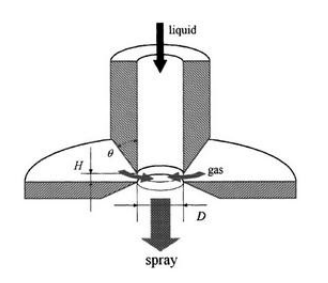
\includegraphics[width=0.6\textwidth]{figures/Inyector2.png}
    \caption{Geometría del Nebulizador Flow Blurring.}
    \label{fig:inyectorEsquema}
\end{figure}

Como se puede observar en la figura \ref{fig:inyectorEsquema}, la geometría se caracteriza con dos magnitudes: la altura $H$ y el diámetro $D$. La relación entre ambas, $\phi = \dfrac{H}{D}$, es un parámetro clave que determina el régimen de nebulización, Flow Focusing o Flow Blurring. Los nebulizadores Flow Blurring poseen una relación $\phi$ menor que $0.5$.

En este tipo de nebulizador neumático, el spray se controla típicamente con presiones ycaudales de gas y líquido. Existe una transferencia de energía (para una presión de gas fija) que se traduce en una presión mínima de líquido capaz de sostener una atomización estable; fuera de esa “ventana” puede aparecer desde spray poco saturado hasta chorro líquido.

\subsection{Obtención de los vídeos de alta velocidad}

Para conseguir captar información de tamaño y velocidades de las gotas se necesita una gran resolución espacial y temporal. Para ello es necesario el uso de cámaras de alta velocidad, en el caso de los experimentos analizados, se ha utilizado una Shimadzu HPV-2 capaz de grabar a 1 millón de fotogramas por segundo (fps). Durante los experimentos se realizan grabaciones cortas de unos 120 frames, variando los intervalos temporales entre frames ($1\mu s$, $2\mu s$, $4\mu s$, ...) y el zoom.

Al aumentar la velocidad de grabación y el zoom, se reduce la cantidad de luz que llega al sensor, lo que hace necesario el uso de un flash de alta intensidad.

El procedimiento de adquisición de los vídeos es el siguiente:
\begin{enumerate}
    \item Montar el sistema de atomización  y posicionar el inyector para capturar en la salida o a una distancia aguas abajo (por ejemplo, 4 cm, mencionada como zona de interés para formación de gotas).
    \item Encender la cámara con antelación (se menciona un calentamiento previo recomendado).
    \item Enfocar usando un patrón (por ejemplo un alambre de diámetro conocido), de forma que el plano enfocado sea el de máxima nitidez.
    \item Repetir enfoque al cambiar el zoom (x1, x3, x6). Este uso del alambre también sirve como calibración geométrica (relación píxel–longitud) si el diámetro del alambre es conocido. 
\end{enumerate}

\vspace*{0,7cm}

\begin{figure}[h] 
    \centering
    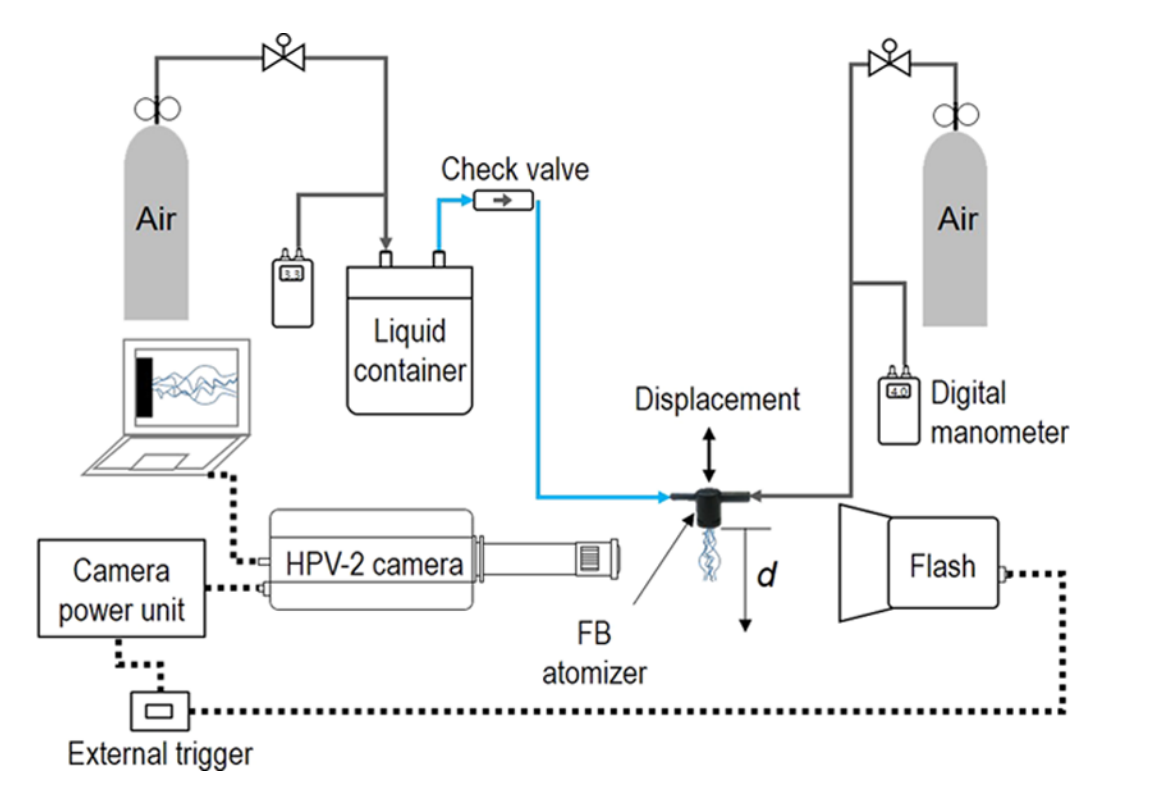
\includegraphics[width=0.8\textwidth]{figures/Exp.png}
    \caption{Montaje experimental para la adquisición de vídeos de alta velocidad.}
    \label{fig:montajeExperimental}
\end{figure}

\section{Introducción al procesamiento de imágenes digitales}\label{sec:intropi}

En esta sección se procederá a dar unas breves pinceladas sobre la representación digital de las imágenes, así como los conceptos básicos del procesamiento de imágenes digitales, que serán necesarios para entender los algoritmos y técnicas que se desarrollarán en los siguientes apartados. Se explicará qué es una imagen digital, cómo se representa y cuáles son las operaciones básicas que se pueden realizar sobre ella.

En este proyecto se trabaja con vídeos de alta velocidad, que no son más que secuencias de imágenes digitales relacionadas temporalmente. Por lo tanto, es fundamental entender cómo se representan las imágenes digitales para poder aplicar técnicas de procesamiento de imágenes y análisis de vídeo.

\subsection{¿Qué es una imagen digital?}

Las imágenes se pueden dividir principalmente en dos tipos: imágenes analógicas e imágenes digitales. Las imágenes analógicas son una representación física de la luz, en la fotografía tradicional, por ejemplo, la luz reacciona con sustancias químicas para formar una imagen. Esta variación química es continua, lo que significa que las transiciones de color o luz fluyen sin interrupciones, formando un gradiente suave sin divisiones exactas. Por otro lado, las imágenes digitales son una representación discreta de la luz, dónde la imagen se divide en una cuadrícula de pequeños elementos numéricos llamados píxeles. Cada píxel tiene un valor que representa la intensidad de la luz (en imágenes en escala de grises) o los valores de color (en imágenes a color). Esta representación discreta permite almacenar, procesar y analizar las imágenes utilizando algoritmos computacionales, como es el caso.

\subsection{Representación de las imágenes digitales}

Para representar una imagen digital, se utiliza una matriz de píxeles. Definamos $p = f(x, y)$, donde $x$ y $y$ son las coordenadas espaciales y $f$ es la función de iluminación que asigna un valor de intensidad (o color) a cada píxel. En el caso de imágenes en escala de grises, cada píxel tiene un valor que representa la intensidad de la luz, típicamente en un rango de 0 a 255, donde 0 representa el negro y 255 representa el blanco. En el caso de imágenes a color, cada píxel se representa mediante tres valores (R, G, B), cada uno en un canal (matriz) diferente que corresponden a las intensidades de los colores rojo, verde y azul, respectivamente \cite{gonzalez2018digital}.

Así que para una imagen digital de tamaño $n x n$, la representación en formato matricial $A$ sería la siguiente:

\begin{equation} \label{eq:matriz}
\mathbf{A} = 
\begin{bmatrix}
f(0,0) & f(0,1) & \dots & f(0,n-1) \\
f(1,0) & f(1,1) & \dots & f(1,n-1) \\
\vdots & \vdots & \ddots & \vdots \\
f(n-1,0) & f(n-1,1) & \dots & f(n-1,n-1)
\end{bmatrix}
\end{equation}

O representada de manera compacta:

\begin{equation} \label{eq:matrizCompacta}
P_{i,j} = f(i, j) ~~~~ i,j \in {0, n-1}
\end{equation}

Una vez definido la forma de representar imágenes digitales, podemos proceder a explicar algunas técnicas clásicas de procesamiento.

\section{Técnicas clásicas}

En este apartado de abordarán de manera teórica los algoritmos y técnicas que se han tenido en cuenta para el desarrollo de este proyecto, iremos desde el preprocesamiento, pasando por la segmentación, operaciones morfológicas y finalmente el tracking de objetos, cubriendo así todo el pipeline de la solución implementada.

\subsection{Preprocesamiento de imágenes}\label{subsec:preproc}

El preprocesamiento de imágenes es una etapa fundamental en el procesamiento de imágenes digitales, ya que permite mejorar la calidad de la imagen y facilitar la posterior segmentación y análisis. En esta sección se describirán las técnicas de reducción de ruido y mejora de contraste que se han considerado para el desarrollo de este proyecto.

\subsubsection{Mejora del contraste}
La idea detrás de la mejora del contraste es aumentar la diferencia entre las intensidades de los píxeles, o lo que es lo mismo, hacer más oscuro lo oscuro y más claro lo claro. Ya que si los frames presentan un histograma de intensidades concentrado en un rango pequeño, la segmentación e identificación de detalles puede resultar difícil. Para solventar este problema se han tenido en cuenta las siguientes técnicas:

\textbf{Ecualización Adaptativa del Histograma con Contraste Limitado (CLAHE):} La ecualización global del histograma puede amplificar el ruido en regiones uniformes, ya que un histograma muy concentrado en pocos valores se estira de forma agresiva al redistribuirse. Por eso, la idea principal de CLAHE \cite{zuiderveld1994clahe} es dividir la imagen en pequeñas regiones (tiles) y aplicar la ecualización del histograma de manera local en cada una de ellas. Además, para evitar la sobreamplificación del ruido, el histograma de cada tile se recorta en un límite de contraste configurable (clip limit), y el exceso se redistribuye uniformemente sobre el resto del histograma. Si no existiese este límite, el ruido se podría amplificar excesivamente; por ejemplo, si una zona de la imagen es homogénea (p.\,ej., un fondo oscuro) y contiene un par de píxeles ruidosos, tras la ecualización esos píxeles, antes imperceptibles, se convertirían en puntos brillantes. Finalmente, para evitar costuras visibles en las fronteras entre tiles, los valores de píxeles cercanos a los bordes se obtienen mediante interpolación bilineal entre los tiles vecinos, logrando así una transición suave y continua.

\textbf{Estiramiento de contraste:} La idea detrás de esta técnica es remapear los valores de intensidad de la imagen al rango completo de valores posibles (0-255 para imágenes en escala de grises). Es decir, hace una transformación lineal que asigna el percentil mínimo ($p_{min}$) de intensidad a 0 y el percentil máximo ($p_{max}$) a 255, estirando proporcionalmente los valores intermedios:

\begin{equation}
I'(x,y) = \frac{I(x,y) - p_{min}}{p_{max} - p_{min}} \cdot 255
\end{equation}

Donde $I(x,y)$ es la intensidad original del píxel en la posición $(x,y)$, y $I'(x,y)$ es la intensidad remapeada. La razón para usar los percentiles en lugar de los valores mínimo y máximo absolutos es que si se usa el mínimo y máximo absolutos, un solo píxel ruidoso extremo puede arruinar el resultado. Por ejemplo, si hay un único píxel con valor 10 y otro con valor 250 por ruido, el estiramiento apenas hace nada porque el rango ya parece amplio. En cambio, usando percentiles (p.\,ej., el 1\% y el 99\%), se ignoran esos valores extremos y se obtiene un estiramiento más representativo del rango real de intensidades en la imagen.

\begin{figure}[p]
    \centering
    \small
    
    \begin{subfigure}[b]{0.32\textwidth}
        \centering
        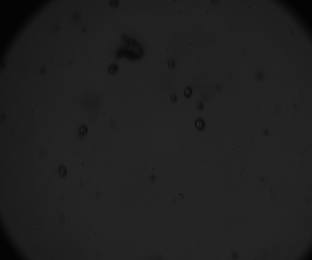
\includegraphics[width=\textwidth]{figures/1_img_original.jpg}
        \caption{Imagen Original (Grises)}
        \label{fig:img_orig}
    \end{subfigure}
    \hfill
    \begin{subfigure}[b]{0.55\textwidth}
        \centering
        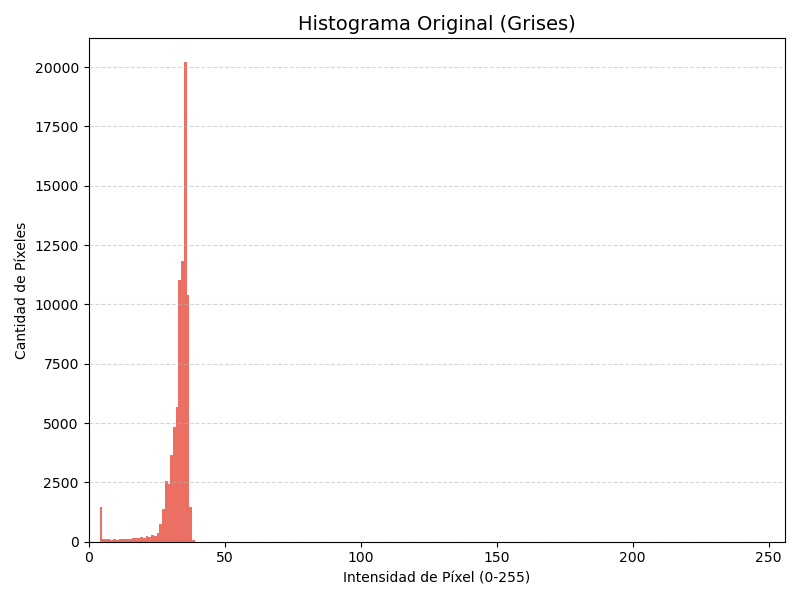
\includegraphics[width=\textwidth]{figures/1_hist_original.png}
        \caption{Histograma Original}
        \label{fig:hist_orig}
    \end{subfigure}
    
    \vspace{0.3cm}
    
    \begin{subfigure}[b]{0.32\textwidth}
        \centering
        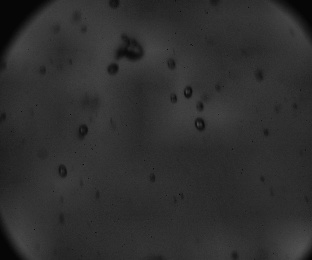
\includegraphics[width=\textwidth]{figures/2_img_clahe.jpg}
        \caption{Imagen con CLAHE}
        \label{fig:img_clahe}
    \end{subfigure}
    \hfill
    \begin{subfigure}[b]{0.55\textwidth}
        \centering
        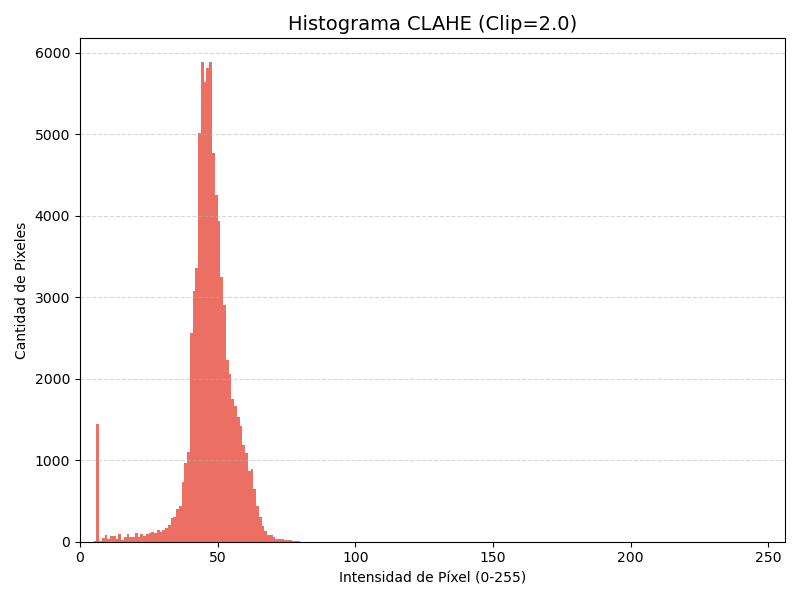
\includegraphics[width=\textwidth]{figures/2_hist_clahe.png}
        \caption{Histograma CLAHE}
        \label{fig:hist_clahe}
    \end{subfigure}
    
    \vspace{0.3cm} 
    
    \begin{subfigure}[b]{0.32\textwidth}
        \centering
        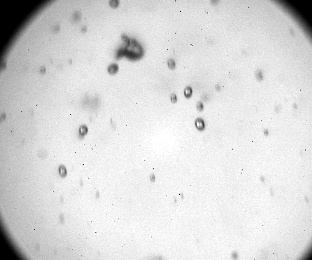
\includegraphics[width=\textwidth]{figures/3_img_estiramiento.jpg}
        \caption{Imagen con Estiramiento}
        \label{fig:img_estir}
    \end{subfigure}
    \hfill
    \begin{subfigure}[b]{0.55\textwidth}
        \centering
        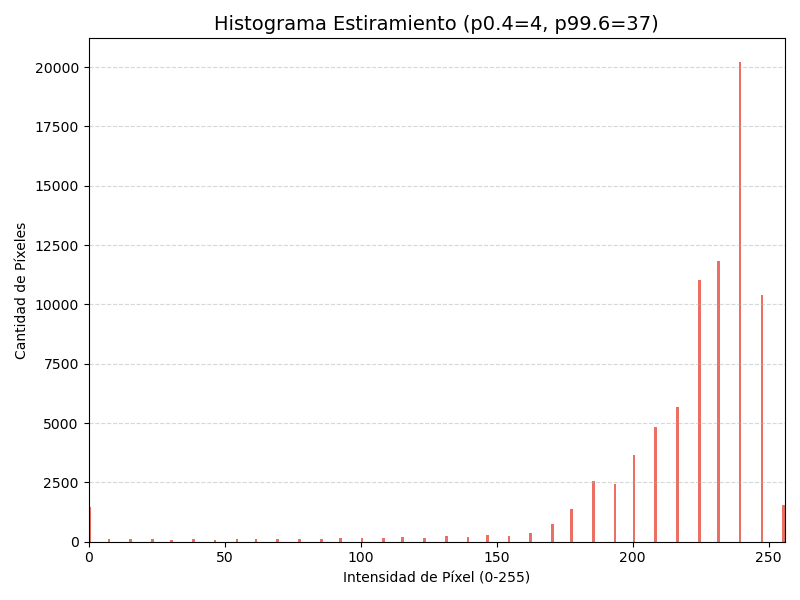
\includegraphics[width=\textwidth]{figures/3_hist_estiramiento.png}
        \caption{Histograma Estiramiento}
        \label{fig:hist_estir}
    \end{subfigure}
    
    \caption{Comparativa de técnicas de mejora: (a-b) Imagen original de bajo contraste; (c-d) Resultado tras aplicar ecualización adaptativa local (CLAHE); (e-f) Resultado tras estiramiento lineal de histograma mediante percentiles.}
    \label{fig:mosaico_histogramas}
\end{figure}

En la figura \ref{fig:mosaico_histogramas} se puede observar un ejemplo de cómo el histograma de la imagen original (con bajo contraste) se concentra en un rango estrecho de intensidades, mientras que tras aplicar CLAHE o estiramiento de contraste, el histograma se distribuye de manera más uniforme a lo largo del rango completo, lo que mejora la visibilidad de los detalles en la imagen.

\subsubsection{Reducción de ruido}

Los procesos de mejora de contraste, especialmente el estiramiento por percentiles, pueden introducir o amplificar ruido de tipo sal y pimienta. Para eliminarlo sin degradar los bordes de las gotas se han considerado los siguientes enfoques:

\paragraph{Filtros de suavizado clásicos:} Uno de los los filtros más comunes en el procesamiento de imágenes es el \textbf{filtro gaussiano}, que convoluciona la imagen con un núcleo gaussiano ($G(x,y,\sigma)$), atenuando las zonas donde hay cambios bruscos de intensidad (como el ruido). El parámetro $\sigma$ controla el grado de suavizado, siendo un valor más alto sinónimo de mayor suavizado. La fórmula que define el peso de cada píxel del núcleo de la convolución es la siguiente:
\begin{equation}
G(x,y,\sigma) = \frac{1}{2\pi\sigma^2} e^{-\frac{x^2 + y^2}{2\sigma^2}}
\end{equation}
En otras palabras, el filtro gaussiano asigna pesos más altos a los píxeles cercanos al centro del núcleo y pesos más bajos a los píxeles más alejados, lo que resulta en un efecto de suavizado que preserva las estructuras generales de la imagen mientras reduce el ruido.
Otro filtro común es el \textbf{filtro de mediana}, que reemplaza cada píxel con la mediana de los valores de los píxeles en su vecindad. Este filtro es especialmente efectivo para eliminar el ruido de tipo sal y pimienta, ya que la mediana no se ve afectada por valores extremos (píxeles ruidosos), a diferencia del promedio que sí puede ser influenciado por ellos.

\paragraph{Fast Non-Local Means Denoising (fNLM):} Los filtros clásicos solo consideran la información de los píxeles cercanos, pero el algoritmo \textbf{fNLM} \cite{ipol.2011.bcm_nlm} asume que una imagen puede tener patrones repetitivos como texturas o zonas lisas, así que toma información de todos los píxeles de la imagen para el suavizado. El algoritmo trabaja con ventanas de píxeles (patches), es decir el algoritmo cogerá una ventana alrededor del píxel a suavizar (el parche $v(N(i))$) y buscará en toda la imagen ventanas similares ($v(N(j))$). La definición matemática es la siguiente:
\begin{equation}
    NL(v) = \frac{1}{C(i)} \sum_{j \in \Omega} e^{-\frac{||v(N_i) - v(N_j)||^2_{2,a}}{h^2}} v(j)
\end{equation}
Donde $NL(v)$ es el nuevo valor que le vamos a dar al píxel $i$, $C(i)$ es un factor de normalización, se divide por la suma total de los pesos. El $\sum_{j \in \Omega} ... v(j)$ Es la suma de los valores de los píxeles $j$ multiplicados por un peso que explicaremos a continuación. $||v(N_i) - v(N_j)||^2_{2,a}$ mide la similitud entre los parches, es decir, la distancia euclídea entre los parches $N_i$ y $N_j$, ponderada por una función gaussiana que da más importancia a los píxeles cercanos al centro del parche. El parámetro $h$ controla el grado de suavizado, siendo un valor más alto sinónimo de mayor suavizado. Esto hace que si el parche $N_j$ es muy similar al parche $N_i$, el peso será alto y el valor de $v(j)$ contribuirá significativamente al nuevo valor de $i$. Por el contrario, si el parche $N_j$ es diferente, el peso será bajo y su contribución será mínima. De esta forma, el algoritmo logra reducir el ruido mientras preserva los detalles y texturas de la imagen. Este algoritmo es fast ya que se restringe la búsqueda de parches similares a una ventana de tamaño $S$ alrededor del píxel $i$, en lugar de buscar en toda la imagen, lo que reduce el orden de complejidad de  $\mathcal{O}(N^2)$ a $\mathcal{O}(N \log N)$, donde $N$ es el número total de píxeles en la imagen.


\subsection{Segmentación de imágenes}\label{subsec:segmentacion}

Segmentación es el proceso de dividir una imagen en regiones o segmentos con significado semantico, en este caso, el objetivo es segmentar las gotas del fondo.

\subsubsection{Umbralización}

La umbralización es una de las técnicas de segmentación más simple, consiste en convertir una imagen en escala de grises en una imagen binaria, donde los píxeles se clasifican como pertenecientes a un objeto (en este caso, una gota) o al fondo, dependiendo de si su intensidad es mayor o menor que un umbral $T$.

En la umbralización global, se elige un único valor de $T$ para toda la imagen. El método \textbf{Otsu} \cite{otsu1979} selecciona automáticamente el umbral que maximiza la varianza entre las clases:
\begin{equation}
    T^{*} = \arg\max_T \left[ w_{0}(T)w_{1}(T)(\mu_{0}(T)-\mu_{1}(T))^2\right]
\end{equation}
Donde $w_{0}(T)$ y $w_{1}(T)$ son las proporciones de las clases de fondo y objeto respectivamente, y $\mu_{0}(T)$ y $\mu_{1}(T)$ son las medias de intensidad de cada clase. Sin embargo, en imágenes con iluminación no uniforme o bajo contraste, la umbralización global puede no ser efectiva, ya que un único umbral puede no separar adecuadamente los objetos del fondo en todas las regiones de la imagen.

Para solucionar este problema, se ha optado por la \textbf{umbralización adaptativa}, en concreto, su versión gaussiana, que calcula un umbral local $T(x,y)$
para cada píxel basado en la media ponderada gaussiana de los píxeles vecinos en una ventana de tamaño $N$ centrada en $(x,y)$, a la que se le resta una constante $C$ para ajustar el umbral:
\begin{equation}
    T(x,y) = \mu_{gauss}(x, y) - C
\end{equation}
El uso de un umbral local asegura la robustez de la segmentación frente a variaciones de iluminación.

\subsubsection{Extracción de contornos}
Una vez binarizada la imagen, los contornos permiten delimitar exactamente cada región segmentada. El algoritmo de \textbf{Suzuki \& Abe} \cite{SUZUKI198532} realiza un recorrido topológico de la imagen binaria etiquetando los bordes exteriores e interiores mediante una única pasada sobre los píxeles, lo que lo hace eficiente en memoria y tiempo. OpenCV expone este algoritmo a través de \texttt{cv2.findContours}, con distintos modos de recuperación (\texttt{RETR\_EXTERNAL} para contornos solo externos, \texttt{RETR\_TREE} para la jerarquía completa) y métodos de aproximación (\texttt{CHAIN\_APPROX\_SIMPLE} para comprimir segmentos rectos, \texttt{CHAIN\_APPROX\_NONE} para devolver todos los puntos).

\subsection{Operaciones morfológicas}

Las operaciones morfológicas operan sobre conjuntos binarios, mediante un elemento estrcuturante (normalmente un cuadrado o un círculo) de forma y tamaño configurable. Las dos operaciones básicas son la dilatación y la erosión, que forman las operaciones compuestas. La \textbf{erosión} elimina píxeles de los bordes de los objetos, lo que puede ayudar a eliminar pequeñas regiones ruidosas o separar objetos conectados. Por otro lado, la dilatación agrega píxeles a los bordes de los objetos, lo que puede ayudar a cerrar pequeños agujeros o conectar objetos cercanos. Combinando estas dos operaciones se puede obtener la apertura y el cierre.

La \textbf{apertura} (opening) es la combinación de erosión seguida de dilatación, lo que elimina objetos más pequeños que el kernel y suaviza los bordes de los objetos más grandes, se suele usar para eliminar ruido del tipo sal y pimienta:
\begin{equation}
 A \circ B = (A \ominus B) \oplus B
\end{equation}
El \textbf{cierre} (closing) es la combinación de dilatación seguida de erosión, lo que cierra pequeños agujeros dentro de los objetos y conecta objetos cercanos, se suele usar para rellenar huecos en los objetos segmentados:
\begin{equation}
 A \bullet B = (A \oplus B) \ominus B
\end{equation}
En la implementación desarrollada se aplica primero la apertura para eliminar el ruido generado por la umbralización, y a continuación el cierre para recuperar la integridad de las gotas que hubieran quedado fragmentadas.

\subsection{Tracking de objetos}

El tracking o seguimiento de objetos en vídeos es el proceso de asociar, frame a frame, las detecciones correspondientes al mismo objeto, construyendo así su trayectoria.

\subsubsection{Flujo óptico de Lucas-Kanade}

El algoritmo de \textbf{Lucas-Kanade} \cite{lucas1981iterative} se basa en la hipótesis de constancia de intensidad, es decir, asume que la intensidad de los píxeles de un objeto se mantiene constante entre frames consecutivos. Para ello, toma una ventana local de píxeles alrededor de cada punto de interés y asume que todos los píxeles de dicha ventana se desplazan de forma uniforme. A continuación, busca en el siguiente frame la posición que minimiza la diferencia de intensidades respecto a la ventana original, obteniendo así el vector de desplazamiento del punto.
Matemáticamente, el algoritmo resuelve la siguiente ecuación para cada punto de interés:
\begin{equation}
    \begin{pmatrix} \sum I_x^2 & \sum I_x I_y \\ \sum I_x I_y & \sum I_y^2 \end{pmatrix}
    \begin{pmatrix} u \\ v \end{pmatrix}
    =
    -\begin{pmatrix} \sum I_x I_t \\ \sum I_y I_t \end{pmatrix}
\end{equation}

donde $(u, v)$ es el vector de desplazamiento que se desea calcular, $I_x$ e $I_y$ son las derivadas parciales de la intensidad de la imagen respecto a $x$ e $y$, respectivamente, y $I_t$ es la derivada parcial respecto al tiempo, es decir, la diferencia de intensidades entre los dos frames.

Este sistema es sobredeterminado: la ecuación básica del flujo óptico $I_x u + I_y v + I_t = 0$ tiene dos incógnitas ($u$ y $v$) pero se aplica a todos los píxeles de la ventana local, generando más ecuaciones que incógnitas. Para obtener una solución única, Lucas-Kanade minimiza la suma de los errores al cuadrado de todas las ecuaciones de la ventana, lo que conduce al sistema matricial $2\times2$ mostrado anteriormente, que sí tiene solución única siempre que la matriz del sistema no sea singular, es decir, siempre que exista suficiente textura en la ventana local.

Sin embargo, la formulación básica falla cuando el desplazamiento entre frames es grande en comparación con el tamaño de la ventana, ya que la hipótesis de desplazamiento uniforme deja de ser válida. Para solventar esto, en la práctica se emplea la \textbf{versión piramidal} del algoritmo \cite{bouguet2001pyramidal}: la imagen se submuestrea en varios niveles de resolución formando una pirámide, se calcula el flujo en el nivel más grueso (donde los grandes desplazamientos se convierten en pequeños) y el resultado se refina progresivamente hacia la resolución original. OpenCV implementa esta variante a través de la función \texttt{cv2.calcOpticalFlowPyrLK}, que es la utilizada en la implementación desarrollada.

\subsubsection{Asignación por distancia mínima}

Una vez predichas las posiciones futuras de los tracks activos mediante flujo óptico, el problema de asociación consiste en decidir qué detección del fotograma actual corresponde a cada track. La estrategia greedy por distancia mínima selecciona para cada detección el track disponible más cercano en términos de distancia euclídea entre centroides, siempre que dicha distancia no supere un umbral máximo configurable. Los tracks que no reciben ninguna detección durante varios fotogramas consecutivos se consideran perdidos y se descartan, mientras que las detecciones sin track asignado generan nuevos tracks.
Este enfoque, combinado con la predicción de Lucas-Kanade, es suficientemente robusto para los vídeos analizados de corta duración ( $\approx$ 120 fotogramas) y con movimiento de gotas relativamente uniforme sin necesidad de recurrir a métodos más complejos como el filtro de Kalman.

\section{Técnicas basadas en deep learning}

Además de los algoritmos clásicos descritos anteriormente, se evaluó la viabilidad de utilizar modelos de segmentación basados en aprendizaje profundo, en particular el modelo \textbf{Segment Anything Model (SAM)} \cite{kirillov2023sam}. SAM es un modelo de segmentación de propósito general entrenado sobre más de mil millones de máscaras anotadas, capaz de segmentar cualquier objeto a partir de prompts en forma de puntos, cajas delimitadoras o máscaras previas. Su arquitectura combina un codificador de imagen basado en \textbf{Vision Transformer (ViT)} con un decodificador ligero de máscaras, lo que le permite generar segmentaciones precisas en una amplia variedad de dominios sin necesidad de reentrenamiento.

Sin embargo, tras las pruebas realizadas en el entorno local, se decidió descartar el uso de SAM como solución final por las siguientes razones: el modelo requiere una GPU con memoria suficiente y una instalación de CUDA, lo que supone una barrera de hardware para los investigadores del departamento. Los tiempos de inferencia por fotograma son significativamente mayores que los de la solución clásica y, en las pruebas realizadas, la ventaja en precisión de segmentación no justificaba el sobrecoste computacional para el tipo de imágenes analizadas, donde las gotas presentan un contraste razonablemente bien definido tras el preprocesamiento. Por estos motivos, se optó por la solución clásica basada en OpenCV, que ofrece un buen equilibrio entre precisión, rendimiento y accesibilidad.
    % LTeX: language=es

\chapter{Planificación y Costes}

\section{Metodología de desarrollo}

El desarrollo de este proyecto ha seguido una textbf{metodología iterativa e incremental}, basada en los principios ágiles del desarrollo de software \cite{beck2001agile}. Se ha decidido adoptar esta metodología en lugar de un enfoque clásico en cascada debido al tipo de proyecto ante el que nos encontramos, que al ser de carácter exploratorio, requiere una gran flexibilidad que permita ir validando hipótesis en cada iteración para ir ajustando el rumbo del desarrollo. Además, al comenzar el proyecto, se tenía claro el objetivo al que se quería llegar, pero no el camino a seguir para alcanzarlo, por este motivo, una metodología en casada no habría sido viable por la rigidez e intolerancia al cambio por la que se caracteriza.

El proyecto se ha planteado con textbf{ciclos cortos de desarrollo} de una o dos semanas de duración, según la dificultad de los obetivos marcados y la carga lectiva de ese periodo, cada uno de ellos estructurado de la siguiente manera:

\begin{itemize}
    \item \textbf{Planificación:} Se definen los objetivos concretos del ciclo (p. ej., implementar la umbralización adaptativa, desarrollar la mejora del tracking, etc.)
    \item \textbf{Implementación:} Se trabaja sobre el código para integrar los nuevos objetivos con el resto de la arquitectura del analizador.
    \item \textbf{Prueba y validación:} Una vez completado el desarrollo del ciclo, se prueban las nuevas funcionalidades para ver si cumplen los objetivos marcados.
    \item \textbf{Revisión:} Se evalúa junto con el tutor el resultado del ciclo, se marcan posibles puntos de mejora y se planifica el siguiente ciclo. Muchas veces en esta fase, se decide tomar un camino diferente en el diseño del analizador, como por ejemplo, descartar el uso de modelos de deep learning para la segmentación de las gotas.
\end{itemize}

Esta metodología ha permitido un contacto estrecho con los tutores del proyecto, que en este caso actúan como \textit{stakeholders} del proyecto, que aportaban retroalimentación desde la perspectiva de investigadores y usuarios finales del analizador. Dicha retroalimentación ha sido especialmente valiosa en muchas decisiones de diseño, como por ejemplo, la inclusión del factor pixel-unidad real, la implementación de la visualización en tiempo real, o la elección de las gráficas que se exportan al finalizar el análisis.

Para gestionar todo el código desarrollado, se ha utilizado Git y GitHub \cite{git_software} \cite{github_platform}, lo que ha permitido llevar un historial de versiones que permitía revertir a versiones anteriores en caso de que alguna nueva funcionalidad introdujera errores o no cumpliera con los objetivos marcados. Además, como el analizador posee una estructura modular, cada nueva funcionalidad se desarrollaba en ramas separadas, para poder probarlas sin interferir con el resto del desarrollo. La memoria del proyecto también se ha gestionado en el mismo repositorio, centralizando documentación y código en un mismo lugar.

\section{Documento de requisitos}

En esta sección se detallarán los requisitos funcionales y no funcionales que se han identificado para el proyecto, fruto de las reuniones con los tutores y del desglose del flujo de trabajo actual del análisis manual de los experimentos del departamento.

En ingeniería de software, se distinguen, principalmente, dos categorías de requisitos principales \cite{sommerville2016}: los \textbf{requisitos funcionales}, que distinguen qué debe hacer el sistema, es decir, las funciones, comportamientos y servicios concretos que tiene que ofrecer la solución implementada; y los \textbf{requisitos no funcionales}, que describen cómo deber ser el sistema, es decir, restricciones sobre calidad, usabilidad, portabilidad o rendimiento, entre otras propiedades que no corresponden a una funcionalidad concreta, pero que determinan igualmente el éxito del proyecto.

\subsection{Requisitos funcionales}

Los requisitos funcionales definen las capacidades que el sistema debe proporcionar al usuario. En este proyecto se han identificado los siguientes:

\begin{itemize}
    \item \textbf{RF-01 Carga de vídeo:} El sistema debe permitir cargar vídeos de alta velocidad en los formatos AVI, MP4, MOV y MKV.
    \item \textbf{RF-02 Calibración espacial:} El sistema debe permitir establecer una factor de conversión píxel-unidad real para poder representar las mediciones en dichas unidades.
    \item \textbf{RF-03 Calibración temporal:} El sistema debe permitir configurar la tasa de frames de adquisición del vídeo, obviando los metadatos del mismo. Esto es crucial para el cálculo de la velocidades.
    \item \textbf{RF-04 Preprocesamiento configurable:} El sistema debe implementar el método de estiramiento de percentiles como mejora del contraste, ya que es el método al que los investigadores están acostumbrado a usar, si se implementa otro método, se debe permitir configurar el método a usar.
    \item \textbf{RF-05 Segmentación de gotas:} El sistema debe segmentar automáticamente las gotas, para su posterior análisis.
    \item \textbf{RF-06 Filtrado de detecciones:} El sistema tiene que implementar un filtrado de detecciones para eliminar falsos positivos, ya que, en muchos vídeos, hay artefactos que pueden ser detectados erróneamente como gotas, como por ejemplo, el marco circular del objetivo de la cámara.
    \item \textbf{RF-07 Tracking de gotas:} El sistema debe implementar un método que permita seguir las gotas a lo largo de los frames, para poder calcular trayectorias y velocidades.
    \item \textbf{RF-08 Cálculo de métricas:} El sistema debe calcular las siguiente métricas para cada gota detectada: diámetro, área, centroide, velocidad, diámetro equivalente, circularidad, perímetro y trayectoria.
    \item \textbf{RF-09 Exportación de datos:} El sistema debe permitir exportar los datos del análisis en formato CSV, permitiendo su posterior análisis por parte de los investigadores con herramientas como Excel o Python.
    \item \textbf{RF-10 Generación de gráficas:} El sistema debe generar un conjunto de gráficas en formato PNG al finalizar el análisis, junto con los datos de cada eje en formato CSV, para permitir que los investigadores puedan editar las gráficas facilmente con otras herramientas como Excel o Python.
    \item \textbf{RF-11 Vídeo de salida:} El sistema debe generar un vídeo en el que se superpongan las detecciones y trayectorias sobre el vídeo original, para poder validar visualmente los resultados.
    \item \textbf{RF-12 Frames de diagnóstico:} El sistema debe permitir previsualizar el resultado del preprocesamiento y la binarización sobre el primer fotograma sin necesidad de ejecutar el análisis completo.
    \item \textbf{RF-13 Previsualización en tiempo real:} Durante el procesamiento, el sistema debe mostrar en una ventana flotante los fotogramas original, preprocesado, binarizado y con tracking superpuesto.
    \item \textbf{RF-14 Cancelación del análisis:} El sistema debe permitir detener el procesamiento de forma segura en cualquier momento.
    \item \textbf{RF-15 Interfaz gráfica de usuario:} El sistema debe contar con una interfaz gráfica de usuario intuitiva y fácil de usar, que permita a los investigadores configurar los parámetros del análisis y visualizar los resultados de forma clara, ya que los investigadores no tienen por que tener conocimientos avanzados de informática y programación.
\end{itemize}

\subsection {Requisitos no funcionales}

Los requisitos no funcionales establecen las restricciones de calidad que debe satisfacer el sistema en su conjunto, independientemente de las funciones que realice. Para este proyecto se han identificado los siguientes:

\begin{itemize}
    \item \textbf{RNF-01 Usabilidad:} La interfaz gráfica debe ser intuitiva y accesible para investigadores sin conocimientos de programación. Todos los parámetros deben poder ajustarse sin editar código.
    \item \textbf{RNF-02 Portabilidad:} La solución debe poder ejecutarse en  Windows sin la necesidad de instalar ninguna dependencia adicional, debe distribuirse como ejecutable (.exe).
    \item \textbf{RNF-03 Arquitectura modular:} El sistema debe ser modular, permitiendo así la integración de nuevas funcionalidades de manera sencilla; y facilitando el mantenimiento y escalabilidad del sistema. Cada fase del pipeline de análisis debe ser implementada como un módulo independiente, que reciba una entrada del módulo anterior y entregue una salida al siguiente módulo.
    \item \textbf{RNF-04 Rendimiento:} la interfaz no se debe bloquear durante el procesamiento. El sistema no tiene que ser en tiempo real, pero debe mostrar el progreso del análisis al usuario.
    \item \textbf{RNF-05 Código abierto:} La solución debe basarse exclusivamente en bibliotecas de código abierto, sin dependencias de software comercial o con licencias restrictivas. Esto es clave para garantizar el acceso gratuito a la herramienta por parte de la comunidad científica.
    \item \textbf{RNF-06 Reproducibilidad:} Dado el mismo vídeo y los mismos parámetros, el sistema debe producir siempre los mismos resultados.
\end{itemize}


\section{Alcance del proyecto}

El alcance de este proyecto comprende el diseño, implementación, validación y documentación de una herramienta de escritorio que segmente, siga y analice automáticamente las gotas de los vídeos de alta velocidad adquiridos en experimentos de nebulización e inyección. A continuación, se detallarán los límites y exclusiones del proyecto.

\subsection{Elementos contemplados}

\begin{itemize}
    \item Desarrollo completo del pipeline de procesamiento de imagen (preprocesamiento, segmentación, filtrado, tracking y exportación).
    \item Desarrollo de la interfaz gráfica de usuario con todos los controles necesarios para configurar y ejecutar el análisis.
    \item Generación automática de gráficas estadísticas y ficheros CSV con los resultados.
    \item Evaluación y descarte motivado de técnicas alternativas basadas en aprendizaje profundo (SAM).
    \item Manual de usuario.
    \item Ejecutable para Windows ( .exe ).
\end{itemize}

\subsection{Elementos excluidos}

\begin{itemize}
    \item \textbf{EX-01 Análisis de resultados de experimentos:} El análisis de los resultados físicos de los experimentos de nebulización (esto corresponde al dominio de los investigadores del departamento).
    \item \textbf{EX-02 Versión web o multiplataforma:} El desarrollo no incluye una versión web o móvil de la herramienta, se centra exclusivamente en una aplicación de escritorio para Windows.
    \item \textbf{EX-03 Integración con el sistema de adquisición de vídeo:} No se contempla la integración en el pipeline de adquisición, los vídeos tendrán que ser cargados manualmente por los investigadores en la aplicación.
    \item \textbf{EX-04 Creación de un dataset de entrenamiento:} No se contempla la creación de un dataset de segmentación para entrenar o reentrenar modelos de deep learning. Esto es debido a la gran cantidad de tiempo que se requeriría para el etiquetado manual de las gotas.
\end{itemize}


\section{Hitos}

Para este proyecto se han definido los siguientes hitos, que marcan la finalización de las etapas principales del diseño y desarrollo del analizador:

\begin{itemize}
    \item \textbf{H-01 Inicio del proyecto (03/03/2025):} Comienzo formal del desarrollo, establecimiento del entorno de trabajo (Python, OpenCV, Git) y análisis de los primeros vídeos de muestra proporcionados por el departamento.
    \item \textbf{H-02 Definición del marco teórico y aproximación al problema (31/08/2025):} Investigación sobre las técnicas de procesamiento de imágenes y visión por computador. Estudiar si enfocar el desarrollo en técnicas clásicas o modelos de deep learning. Básicamente, adquirir los conocimientos necesarios para implementar una solución fundamentada y eficaz.
    \item \textbf{H-03 Pipeline básico y funcional (30/11/2025):} Implementación básica del pipeline de preprocesado, segmentación, mediciones y exportación. Sin interfaz gráfica ni tracking, pero con un flujo de trabajo funcional que permita procesar vídeos y obtener resultados.
    \item \textbf{H-04 Interfaz gráfica de usuario (31/12/2025):} Desarrollo de una primera versión de la interfaz gráfica, que permita ejecutar el pipeline básico de análisis desde una aplicación de escritorio.
    \item \textbf{H-05 Implementación del tracking (28/02/2026):} Integrar el tracking y la medición de velocidades en el pipeline.
    \item \textbf{H-06 Pruebas y ajustes finales (31/03/2026):} Probar el sistema para validar que cumple los requisitos y objetivos marcados, ajustar parámetros y corregir errores.
    \item \textbf{H-07 Memoria y entrega final (27/05/2026):} Redacción de la memoria del proyecto y entrega final de la aplicación.
\end{itemize}

\section{Desglose de tareas (EDT)}

La \textbf{Estructura de Desglose del Trabajo} (EDT, o \textit{Work Breakdown Structure} en inglés) es una herramienta de gestión de proyectos que descompone el trabajo total en unidades más pequeñas y manejables, organizadas de forma jerárquica \cite{pressman2014}. El objetivo de la EDT no es describir \textit{cómo} se realiza el trabajo, sino \textit{qué} hay que hacer. Esta descomposición facilita la estimación del esfuerzo y el seguimiento del avance a lo largo del desarrollo.

En este proyecto la EDT se ha estructurado en tres niveles: el nivel raíz representa el proyecto en su conjunto, el segundo nivel agrupa el trabajo en cinco bloques funcionales (T1-T5) y el tercer nivel desglosa cada bloque en subtareas concretas y acotadas. La Figura~\ref{fig:edt} muestra el árbol de desglose completo, donde puede apreciarse que el grupo T2 (\textit{Backend}) es el de mayor número de subtareas, lo que refleja que el pipeline de procesamiento de imagen es la parte más extensa y compleja del desarrollo.

\begin{figure}[H]
    \centering
    \includegraphics[width=\textwidth]{figures/edt.png}
    \caption{Estructura de Desglose del Trabajo (EDT) del proyecto.}
    \label{fig:edt}
\end{figure}

A continuación, se describirán con más detalle cada una de los bloques y sus subtareas.

\subsection{T1: Estudio del estado del arte}

\begin{itemize}
    \item \textbf{T1.1} Revisión bibliográfica de técnicas de procesamiento de imágenes digitales.
    \item \textbf{T1.2} Análisis de herramientas comerciales existentes (LaVision, Dantec Dynamics) e identificación de sus limitaciones.
    \item \textbf{T1.3} Exploración de técnicas de deep learning (SAM) y evaluación de su viabilidad para este proyecto en concreto.
    \item \textbf{T1.4} Familiarización con OpenCV y las librerías de Python necesarias para el análisis de imágenes y visión por computador.
\end{itemize}

\subsection{T2: Desarrollo del backend}
\begin{itemize}
    \item \textbf{T2.1} Diseño de la arquitectura modular del pipeline y de la clase \texttt{DropletAnalyzer}.
    \item \textbf{T2.2} Módulo de preprocesamiento: escala de grises, mejora de contraste y reducción de ruido.
    \item \textbf{T2.3} Módulo de segmentación: umbralización adaptativa gaussiana y operaciones morfológicas (apertura y cierre).
    \item \textbf{T2.4} Módulo de filtrado y medición: filtros de área y circularidad, cálculo de centroide, diámetro equivalente, redondez y bounding box.
    \item \textbf{T2.5} Módulo de tracking: flujo óptico de Lucas-Kanade combinado con asignación greedy por distancia euclídea mínima.
    \item \textbf{T2.6} Módulo de cálculo de velocidades.
    \item \textbf{T2.7} Módulo de exportación de resultados a CSV y generación de gráficas (\texttt{DropletPlotter}).
\end{itemize}

\subsection{T3: Desarrollo del frontend}
\begin{itemize}
    \item \textbf{T3.1} Diseño de la arquitectura de la interfaz gráfica con Tkinter y definición de los controles de cada parámetro.
    \item \textbf{T3.2} Implementación de la ventana principal: las seis secciones, sliders con campos de entrada y botones de reset.
    \item \textbf{T3.3} Implementación del sistema de hilos (\texttt{threading}) y colas (\texttt{queue}) para desacoplar procesamiento e interfaz.
    \item \textbf{T3.4} Implementación de la ventana flotante de previsualización en tiempo real con los cuatro paneles.
    \item \textbf{T3.5} Integración del frontend con el backend a través de la API pública de \texttt{DropletAnalyzer} y \texttt{DropletPlotter}.
\end{itemize}

\subsection{T4: Pruebas y ajuste de parámetros}
\begin{itemize}
    \item \textbf{T4.1} Pruebas sobre los vídeos reales de los experimentos con nebulizadores.
    \item \textbf{T4.2} Ajuste iterativo de los valores por defecto de los parámetros para cubrir la mayor variedad posible de condiciones de grabación.
    \item \textbf{T4.3} Validación visual del tracking comparando el vídeo de salida con los fotogramas originales.
\end{itemize}

\subsection{T5: Documentación}
\begin{itemize}
    \item \textbf{T5.1} Redacción de la memoria del TFG.
    \item \textbf{T5.2} Elaboración del manual de usuario (\ref{cap:manual_usuario}).
\end{itemize}

\section{Planificación temporal}

La planificación temporal recoge la distribución en el tiempo de las tareas definidas en la EDT y los hitos del proyecto. Para su elaboración se ha utilizado \textbf{Microsoft Project} \cite{microsoft_project}, herramienta estándar en la gestión de proyectos que permite construir diagramas de Gantt, asignar duraciones y dependencias entre tareas, y visualizar la ruta crítica del proyecto. El diagrama resultante se muestra en la Figura.
 
Dado que la metodología adoptada es iterativa, la planificación no es completamente lineal: algunas tareas se solapan en el tiempo o se retoman en iteraciones posteriores a medida que los resultados de las pruebas orientan el desarrollo. No obstante, el diagrama de Gantt refleja una estimación razonable de la dedicación real a cada grupo de tareas a lo largo del periodo de desarrollo del proyecto.


\section{Estudio económico y presupuesto}

\section{Análisis de riesgos}
    \chapter{Implementación}\label{cap:implementacion}

En este apartado se describirá la solución final implementada, detallando tanto el pipeline de procesamiento de imágenes, como la interfaz gráfica desarrollada junto con una breve guía de uso. Para ello, se dividirá el capítulo en dos secciones: una dedicada al backend y otra al frontend.

\section{Backend}

El backend de la aplicación se encarga de procesar las imágenes de alta velocidad obtenidas durante los experimentos con nebulizadores Flow Blurring. Para ello, se ha desarrollado un pipeline de procesamiento que incluye varias etapas, como la preprocesamiento de las imágenes, la segmentación de las gotas y la extracción de características relevantes para el análisis.

Cabe destacar que la mayor parte del esfuerzo de implementación se ha centrado en el desarrollo de este pipeline de procesamiento, ya que es la parte más crítica y compleja de la aplicación. Se han utilizado diversas técnicas de procesamiento de imágenes, como filtros de suavizado, umbralización adaptativa y algoritmos de detección de bordes, para lograr una segmentación precisa de las gotas.

\subsection{Arquitectura del Analizador}

El procesamiento de imágenes se ha implementado en una clase llamada \texttt{DropletAnalyzer}, que se encarga de recibir un vídeo de alta velocidad, procesar cada uno de sus frames y extraer las características relevantes de las gotas presentes en cada frame. El resultado final se almacena en un formato estructurado que puede ser utilizado para análisis posteriores.

Dicha clase se ha diseñado de forma modular, permitiendo la fácil incorporación de nuevas técnicas de procesamiento o la modificación de las existentes sin afectar al resto del pipeline. Esto dota a la aplicación de una gran flexibilidad, permitiendo seleccionar diferentes técnicas de preprocesamiento o segmentación según las características específicas de los vídeos a analizar. Es decir, podríamos definir el pipeline como una cadena de bloques que reciben un frame, ejecutan una acción sobre él y lo pasan al siguiente bloque, de forma que cada bloque es independiente del resto y se pueden modificar o sustituir sin afectar a los demás. La figura \ref{fig:diagramaPipeline} muestra un diagrama de alto nivel donde se pueden diferenciar las distintas etapas (los bloques) por las que pasa cada frame del vídeo hasta obtener el resultado final.

\begin{figure}[ht] 
    \centering
    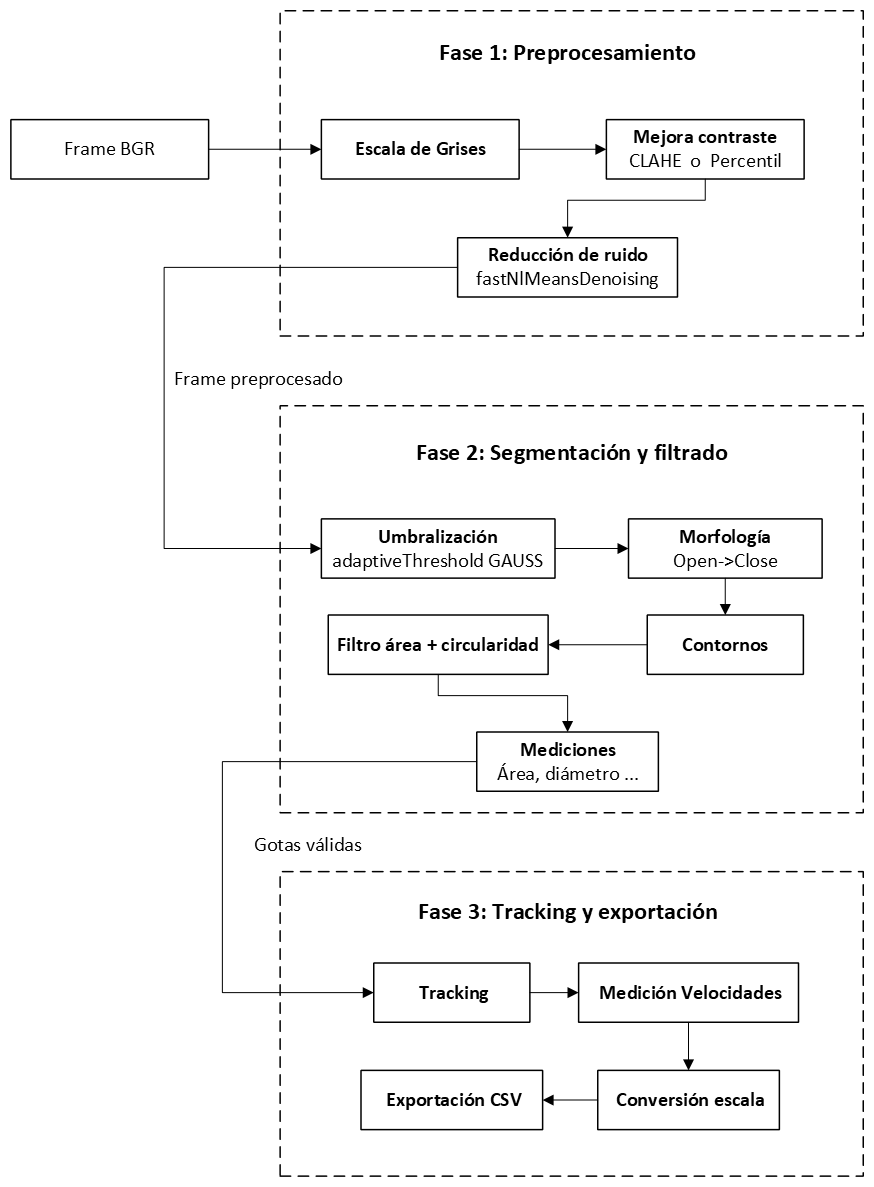
\includegraphics[width=1\textwidth]{figures/Diagrama1.png}
    \caption{Diagrama del pipeline de procesamiento.}
    \label{fig:diagramaPipeline}
\end{figure}

\FloatBarrier

También se han tenido que definir tres tipos de datos (diccionarios) para poder almacenar los parámetros que el usuario puede configurar en la interfaz gráfica, los resultados del procesamiento de cada frame y los resultados finales, una vez terminado el tracking. En la figura \ref{fig:diagramaClaseAn} se muestra un diagrama de la clase \texttt{DropletAnalyzer}, donde se pueden observar los atributos que almacenan estos datos, así como los métodos principales que se encargan de ejecutar cada una de las etapas del pipeline de procesamiento.

\subsection{Preprocesamiento}

El preprocesamiento de los frames del vídeo es la primera etapa del pipeline implementado. En esta etapa se aplican diversas técnicas para mejorar la calidad del contraste y la reducción de ruido en las imágenes, facilitando así la posterior segmentación de las gotas.

Como se pude apreciar en el diagrama de la figura \ref{fig:diagramaPipeline}, el preprocesamiento se compone de tres etapas principales: la conversión a escala de grises, la mejora del contraste y la reducción de ruido. Veamos cada uno de estos bloques con más detalle.

\subsubsection{Conversión a escala de grises}

Como vimos en la sección \ref{sec:intropi}, las imágenes pueden estar compuestas por múltiples canales de color, en nuestro caso, los vídeos de alta velocidad están en formato RGB, aunque el vídeo se vea en blanco y negro. Al pasar de los tres canales RGB de los frames originales a un canal de escala de grises, se simplifica el procesamiento y se reduce la cantidad de información a manejar. Además los algoritmos de detección de bordes usados pasan internamente las imágenes a escala de grises, por lo que no estamos perdiendo ninguna información.

Para realizar esta transformación se usa la función \texttt{cv2.cvtColor} de OpenCV. En las siguientes figuras se muestra el antes y después de la conversión, aunque a simple vista  es difícil apreciar la diferencia.

\begin{figure}[ht]
    \centering
    \begin{subfigure}[t]{0.35\textwidth}
        \centering
        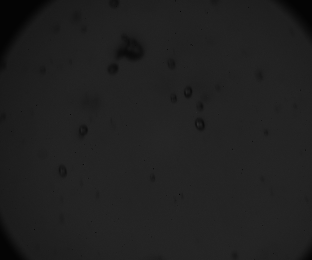
\includegraphics[width=\textwidth]{figures/frameoriginal.png}
        \caption{Original}  
        \label{subfig:original}
    \end{subfigure}
    \hfill
    \begin{subfigure}[t]{0.35\textwidth}
        \centering
        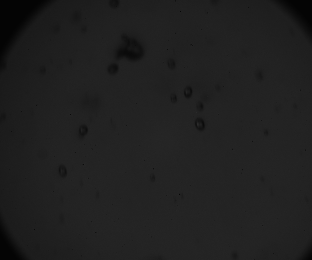
\includegraphics[width=\textwidth]{figures/escaladegrises.png}
        \caption{Gray}  
        \label{subfig:gris}
    \end{subfigure}
    
    \caption{Conversión a escala de grises.}
    \label{fig:preproc-gris}
\end{figure}
\FloatBarrier
\begin{figure}[ht] 
    \centering
    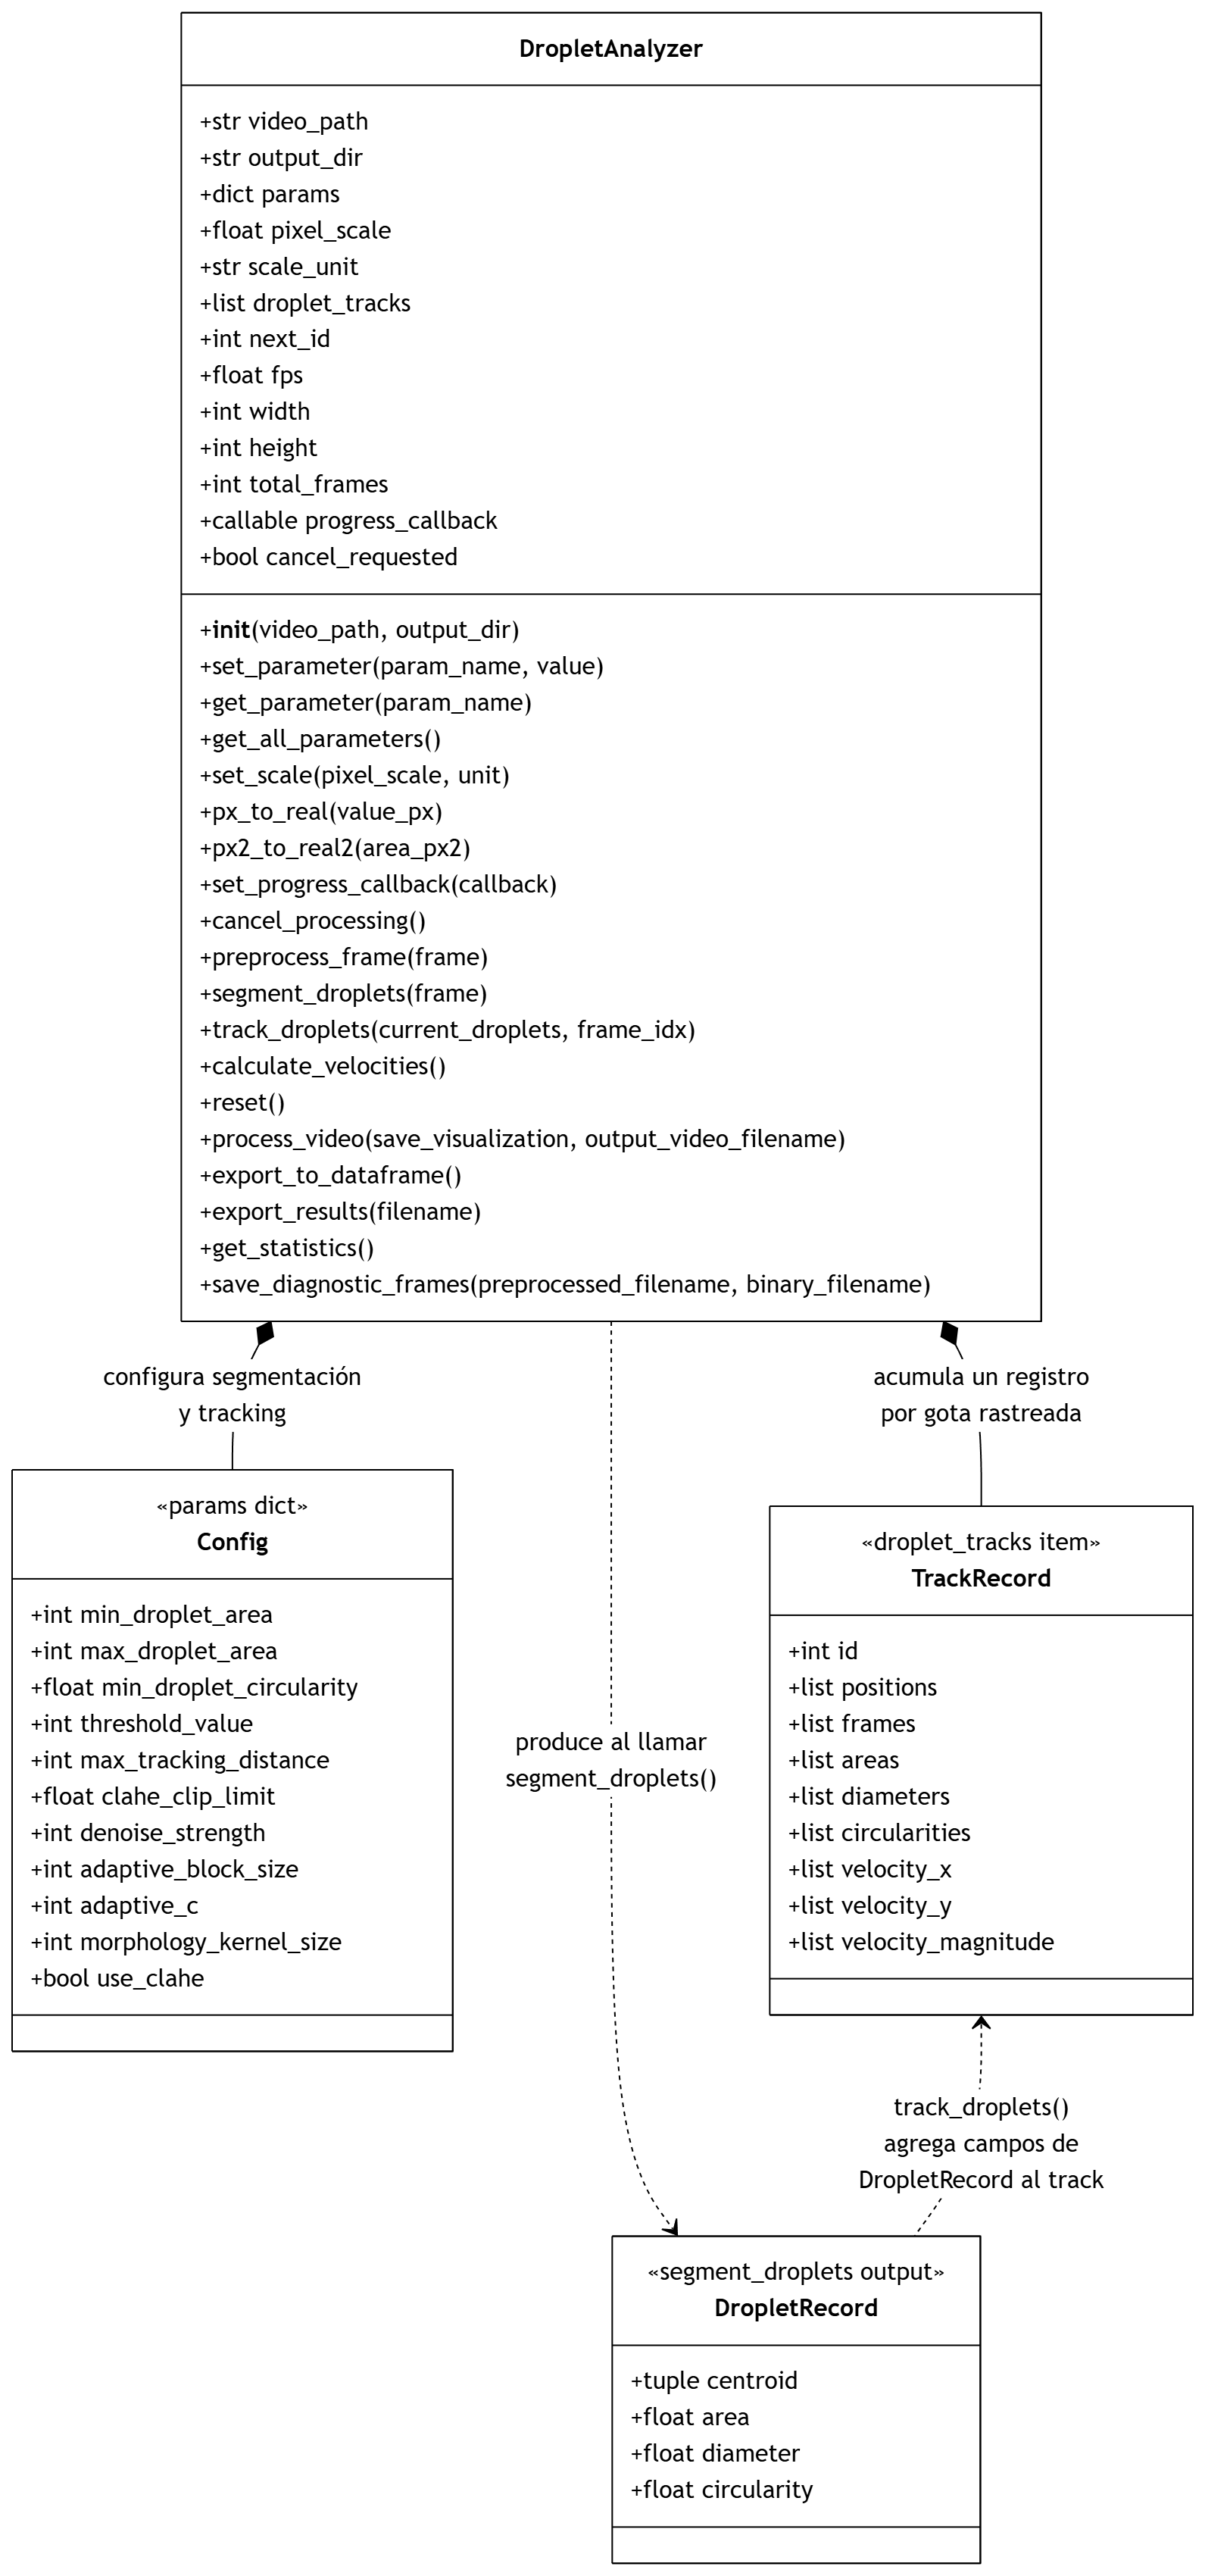
\includegraphics[width=0.7\textwidth]{figures/DiagramaClaseAn.png}
    \caption{Diagrama de la clase DropletAnalyzer.}
    \label{fig:diagramaClaseAn}
\end{figure}
\FloatBarrier

\subsubsection{Mejora del contraste}

Gran parte de los frames capturados durante los experimentos presentan un bajo contraste, como se puede apreciar en la figura \ref{subfig:original}. Para mejorar esto, se han implementado dos técnicas que trabajan sobre sus histogramas: La ecualización adaptativa del histograma (CLAHE) \cite{zuiderveld1994clahe} y el estiramiento del histograma. La teoría detrás de estas técnicas se explicó en la sección \ref{subsec:preproc}, por lo que aquí nos centraremos en su implementación y resultados.

Para la implementación de CLAHE se ha usado la función \texttt{cv2.createCLAHE} de OpenCV, que permite configurar el tamaño de los tiles y el límite de contraste. En el caso del estiramiento del histograma, se ha implementado una función personalizada que ignora el 0.4\% de los píxeles más oscuros y el 0.4\% de los píxeles más claros, estirando el rango de intensidad entre estos percentiles.

El usuario tiene la capacidad de seleccionar entre estas dos técnicas de mejora de contraste y modificar algunos de sus parámetros desde la interfaz gráfica.

La implementación es la siguiente:
\\
\begin{lstlisting}[language=Python, caption={Implementación de mejora de contraste mediante CLAHE y estiramiento por percentiles.}, label={lst:mejora-contraste}]
if self.params['use_clahe']:
    clh = cv2.createCLAHE(
        clipLimit=self.params['clahe_clip_limit'], 
        tileGridSize=(8, 8)
    )
    enhanced = clh.apply(gray)

else:
    flattened = gray.flatten()
    low_percentile = 0.4
    high_percentile = 100.0 - 0.4
    low_val, high_val = np.percentile(flattened, [low_percentile, high_percentile])
    dst = np.clip(gray, low_val, high_val)
    enhanced = ((dst - low_val) / (high_val - low_val) * 255).astype(np.uint8)
\end{lstlisting}

\begin{figure}[ht]
    \centering

    \begin{subfigure}[b]{0.45\textwidth}
        \centering
        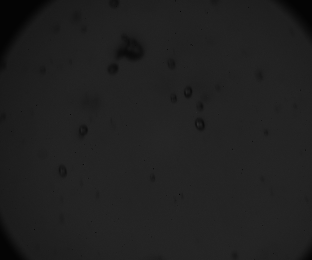
\includegraphics[width=\textwidth]{figures/frameoriginal.png}
        \caption{Original}
        \label{fig:original}
    \end{subfigure}
    \vspace{20pt} 
    \begin{subfigure}[b]{0.45\textwidth}
        \centering
        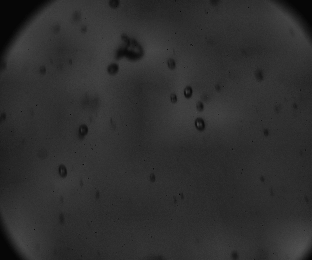
\includegraphics[width=\textwidth]{figures/CLAHE.png}
        \caption{CLAHE}
        \label{fig:CLAHE}
    \end{subfigure}
    \hfill 
    \begin{subfigure}[b]{0.45\textwidth}
        \centering
        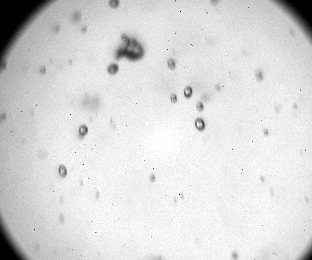
\includegraphics[width=\textwidth]{figures/contrasteporpercentil.png}
        \caption{Estiramiento del histograma}
        \label{fig:estiramiento}
    \end{subfigure}
    \caption{Comparación de técnicas de mejora de contraste.}
    \label{fig:mejora-contraste}
\end{figure}

En la figura \ref{fig:mejora-contraste} se puede apreciar la mejora del contraste obtenida con ambas técnicas. También se puede observar claramente que el estiramiento por percentiles es más agresivo, lo que puede ser beneficioso para algunos vídeos, pero también introduce más ruido, mientras que CLAHE es más suave y puede ser preferible para vídeos con menos problemas de contraste. Por otro lado, se puede apreciar que CLAHE se aplica de manera local, lo que genera esas pequeñas regiones más claras alrededor de las gotas, mientras que el estiramiento por percentiles se aplica de manera global, generando un fondo más uniforme.

\subsubsection{Reducción de ruido}

Tras aplicar las técnicas de mejora de contraste, se introduce algo de ruido de tipo sal y pimienta, como se puede apreciar en \ref{sub@fig:estiramiento}. Para reducir este ruido se ha optado por el uso del algoritmo Fast Non-Local Means Denoising \cite{ipol.2011.bcm_nlm}, implementado en OpenCV a través de la función \texttt{cv2.fastNlMeansDenoising}. Este algoritmo es una versión optimizada del algoritmo Non-Local Means, que reduce el ruido preservando los bordes y detalles de la imagen. El usuario puede configurar el parámetro de fuerza de reducción de ruido desde la interfaz gráfica, permitiendo ajustar el nivel de suavizado según las características específicas de cada vídeo. La teoría detrás de este algoritmo y de otras técnicas de reducción de ruido se explicaron en la sección \ref{subsec:preproc}.

Hay que remarcar que este paso es uno de los más complejos computacionalmente, pero dado que la solución no necesita ser en tiempo real, se ha optado por sacrificar algo de rendimiento a cambio de una mejor calidad en la segmentación de las gotas.

\begin{figure}[ht]
    \centering
    \begin{subfigure}[t]{0.45\textwidth}
        \centering
        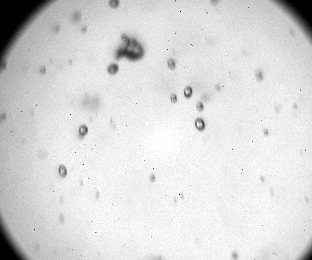
\includegraphics[width=\textwidth]{figures/contrasteporpercentil.png}
        \caption{Ruidosa tras estiramiento}  
        \label{subfig:originalDenoising}
    \end{subfigure}
    \hfill
    \begin{subfigure}[t]{0.45\textwidth}
        \centering
        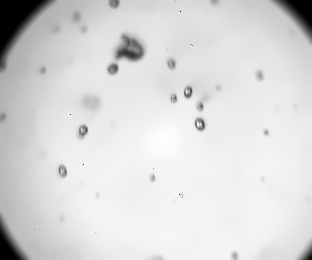
\includegraphics[width=\textwidth]{figures/denoisingNlMeans.png}
        \caption{Denoised}  
        \label{subfig:denoised}
    \end{subfigure}
    
    \caption{Reducción de ruido mediente FNL means Denoising ($h=10$).}
    \label{fig:denoising}
\end{figure}

Como se puede apreciar en la figura \ref{fig:denoising}, el algoritmo FNL means Denoising es capaz de reducir el ruido introducido por el estiramiento del histograma, preservando los bordes y detalles de las gotas. Sin embargo, también se puede observar que se pierde algo de detalle en las gotas más pequeñas, pero en general, las gotas enfocadas de mayor tamaño preservan su forma y bordes.

\subsection{Segmentación y filtrado}

Como se puede apreciar en el diagrama de la figura \ref{fig:diagramaPipeline}, esta etapa es la que conlleva un mayor número de pasos, y podríamos decir que es la etapa central del pipeline de procesamiento, ya que es la encargada de segmentar las gotas presentes en cada frame y extraer las características relevantes para el análisis posterior. En esta sección se describirán los algoritmos y técnicas seleccionados para cada uno de los bloques que componen esta etapa, así como los resultados obtenidos.

\subsubsection{Umbralización}

En este punto nos encontramos con una imagen preprocesada en escala de grises. Para conseguir segmentar las gotas necesitamos diferenciar los píxeles que pertenecen a las gotas de los que pertenecen al fondo. Para ello, se ha implementado una umbralización adaptativa gaussiana, que nos devuelve un frame binarizado, donde los píxeles blancos (255) corresponden a gotas y los píxeles negros (0) corresponden al fondo. 

De todas los algoritmos de umbralización explicados en \ref{subsec:segmentacion}, se ha escogido la umbralización por media local gaussiana, gracias a que al ser local, es mucho más robusta en imágenes que no poseen las mismas condiciones de iluminación en todas las regiones.

La implementación de este método se ha realizado utilizando el método \texttt{adaptiveThreshold} de la biblioteca OpenCV, tomando los parámetros de tamaño de bloque y C de la interfaz de usuario.
\\
\begin{lstlisting}[language=Python, caption=Implementación de Umbralización Adaptativa Gaussiana en OpenCV]
binary = cv2.adaptiveThreshold(
    denoised, 255,
    cv2.ADAPTIVE_THRESH_GAUSSIAN_C,
    cv2.THRESH_BINARY_INV,
    params['adaptive_block_size'],
    params['adaptive_c']
)
\end{lstlisting}

En la figura \ref{fig:thresholding} se puede apreciar el resultado de aplicar esta técnica, hay que destacar que, aún habiendo aplicado un proceso de denoising previo, se sigue observando algo de ruido de tipo sal y pimienta que se eliminará en los siguientes pasos. Quitando el ruido, se puede apreciar que las gotas enfocadas de mayor tamaño se segmentan correctamente, aunque las gotas más pequeñas y desenfocadas no se segmentan tan bien, lo que es un problema común en este tipo de vídeos. Sin embargo, el objetivo de esta etapa no es conseguir una segmentación perfecta, sino una segmentación lo suficientemente buena como para poder extraer características relevantes de las gotas y realizar un seguimiento posterior.

\begin{figure}[ht]
    \centering
    \begin{subfigure}[t]{0.45\textwidth}
        \centering
        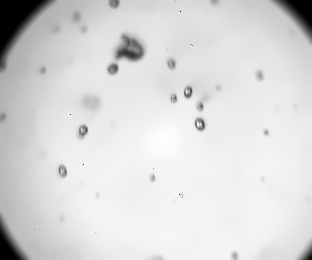
\includegraphics[width=\textwidth]{figures/denoisingNlMeans.png}
        \caption{Denoised}  
        \label{subfig:originalBinary}
    \end{subfigure}
    \hfill
    \begin{subfigure}[t]{0.45\textwidth}
        \centering
        
\includegraphics[width=\textwidth]{figures/bin.png}
        \caption{Binarizada}  
        \label{subfig:bin}
    \end{subfigure}
    
    \caption{Resultados de la umbralización adaptativa gaussiana.}
    \label{fig:thresholding}
\end{figure}

\subsubsection{Operaciones morfológicas}

Tras la umbralización, se han aplicado una serie de operaciones morfológicas para eliminar el ruido de tipo sal y pimienta presente en la imagen binarizada, así como para cerrar pequeños agujeros presentes en las gotas segmentadas. Para ello, se han implementado dos operaciones morfológicas: la apertura y el cierre, utilizando un kernel de forma elíptica de tamaño configurable desde la interfaz gráfica. La apertura se encarga de eliminar el ruido de tipo sal y pimienta, mientras que el cierre se encarga de cerrar pequeños agujeros presentes en las gotas segmentadas, mejorando así la calidad de la segmentación.
La implementación de estas operaciones se ha realizado utilizando la función \texttt{cv2.morphologyEx} de OpenCV, aplicando primero la apertura y luego el cierre.

El usuario puede configurar el tamaño del kernel utilizado en estas operaciones desde la interfaz gráfica, permitiendo ajustar el nivel de eliminación de ruido y cierre de agujeros según las características específicas de cada vídeo. Para ver la teoría detrás de estas operaciones morfológicas, se puede consultar \ref{subsec:segmentacion}.
\\
\begin{figure}[ht]
    \centering
    \begin{subfigure}[b]{0.45\textwidth}
        \centering
        
\includegraphics[width=\textwidth]{figures/bin.png}
        \caption{Binarizada}
        \label{fig:BinMorf}
    \end{subfigure}
    \hfill 
    \begin{subfigure}[b]{0.45\textwidth}
        \centering
        
\includegraphics[width=\textwidth]{figures/OPEN.png}
        \caption{Open}
        \label{fig:open}
    \end{subfigure}
    \vspace{20pt} 
    \begin{subfigure}[b]{0.45\textwidth}
        \centering
        
\includegraphics[width=\textwidth]{figures/CLOSE.png}
        \caption{Close}
        \label{fig:close}
    \end{subfigure}
    \caption{Resultados de las operaciones morfológicas.}
    \label{fig:morfologia}
\end{figure}

En la figura \ref{sub@fig:open} se aprecia que se ha limpiado gran parte del ruido tipo sal y pimienta, aunque también se abren pequeños huecos en la superficie de las gotas fruto de la erosión causada por la apertura. Dichos huecos se vuelven a cerrar tras aplicar la operación de cierre, como se aprecia en la figura \ref{sub@fig:close}.

\subsubsection{Extracción de contornos}

Una vez tenemos una imagen binarizada y lo más limpia posible, el siguiente paso es extraer los contornos de las gotas segmentadas. Para ello, se ha utilizado dos pasadas de la función \texttt{cv2.findContours} de OpenCV, que implementa el algoritmo de Suzuki \& Abe \cite{SUZUKI198532}, explicado en la sección \ref{subsec:segmentacion}.

En la primera pasada, se detectan los contornos de las gotas y se rellenan dichos contornos para obtener una máscara binaria rellena, que se utiliza para eliminar los huecos internos de las gotas segmentadas. En esta pasada se ha optado por usar el modo de recuperación de contornos \texttt{cv2.RETR\_EXTERNAL}, que solo recupera los contornos externos, ya que no nos interesa recuperar los contornos internos de las gotas, y el método de aproximación de contornos \texttt{cv2.CHAIN\_APPROX\_SIMPLE}, que comprime los contornos eliminando los puntos redundantes, ya que no necesitamos una representación exacta de los contornos en esta etapa, sino una representación aproximada que nos permita rellenar las gotas segmentadas.

En la segunda pasada, se vuelven a detectar los contornos sobre la máscara rellena, obteniendo así los contornos finales de las gotas segmentadas, que se utilizan para extraer las características relevantes de cada gota.
En esta pasada se ha optado por usar de nuevo el modo de recuperación de contornos \texttt{cv2.RETR\_EXTERNAL}, y el método de aproximación de contornos \texttt{cv2.CHAIN\_APPROX\_NONE}, que devuelve todos los puntos del contorno sin comprimir, ya que en esta etapa necesitamos una representación exacta de los contornos para poder extraer las características relevantes de cada gota.

\begin{figure}[ht]
    \centering
    \begin{subfigure}[b]{0.45\textwidth}
        \centering
        
\includegraphics[width=\textwidth]{figures/CLOSE.png}
        \caption{Close}
        \label{fig:closeCont}
    \end{subfigure}
    \hfill 
    \begin{subfigure}[b]{0.45\textwidth}
        \centering
        
\includegraphics[width=\textwidth]{figures/cont1.png}
        \caption{Pasada de rellenado}
        \label{fig:filling}
    \end{subfigure}
    \vspace{20pt} 
    \begin{subfigure}[b]{0.45\textwidth}
        \centering
        
\includegraphics[width=\textwidth]{figures/cont2.png}
        \caption{Contornos finales}
        \label{fig:finalContours}
    \end{subfigure}
    \caption{Resultados de la extracción de contornos.}
    \label{fig:contornos}
\end{figure}

En la figura \ref{fig:contornos} se puede apreciar el resultado de la extracción de contornos. En la primera pasada, se detectan los contornos de las gotas segmentadas y se rellenan dichos contornos para obtener una máscara binaria rellena, que se muestra en la figura \ref{sub@fig:filling}. En la segunda pasada, se vuelven a detectar los contornos sobre la máscara rellena, obteniendo así los contornos finales de las gotas segmentadas, que se muestran en la figura de color naranja \ref{sub@fig:finalContours}.

\subsubsection{Filtro de área y circularidad}

En este paso se aplican dos filtros para eliminar los contornos que no corresponden a gotas, basándose en el área y la circularidad de los contornos detectados. 

\FloatBarrier
\section{Frontend}

    \chapter{Manual de Usuario} \label{cap:manual_usuario}

En este capítulo se proporciona un manual de usuario para la aplicación desarrollada, se explicará cómo ejecutar el pipeline completo de manera sencilla. Para obtener más información técnica sobre la implementación, se recomienda revisar los capítulos anteriores.

Para ejecutar la aplicación, simplemente hay que clickar en el archivo ejecutable \texttt{droplet\_analyzer.exe}.

\section{Interfaz Gráfica: Visión General}

Como se vió en el apartado 4.2.2 Descripción de la interfaz \ref{subsec:descripcion_interfaz}, la ventana principal se divide en seis secciones principales:
\begin{itemize}
    \item Sección 1 - Cargar Video: selección del fichero de vídeo de entrada.
    \item Sección 2 - Calibración: conversión de píxeles a unidades reales y ajuste de FPS.
    \item Sección 3 - Nombres de Salida: personalización de los nombres de los archivos generados.
    \item Sección 4 - Parámetros de Procesamiento: ajuste de todos los umbrales y filtros del algoritmo.
    \item Sección 5 - Procesamiento: botones de acción, barra de progreso.
    \item Sección 6 - Log de procesamiento y estadísticas.
\end{itemize}
    
\begin{figure}[H]
    \centering
    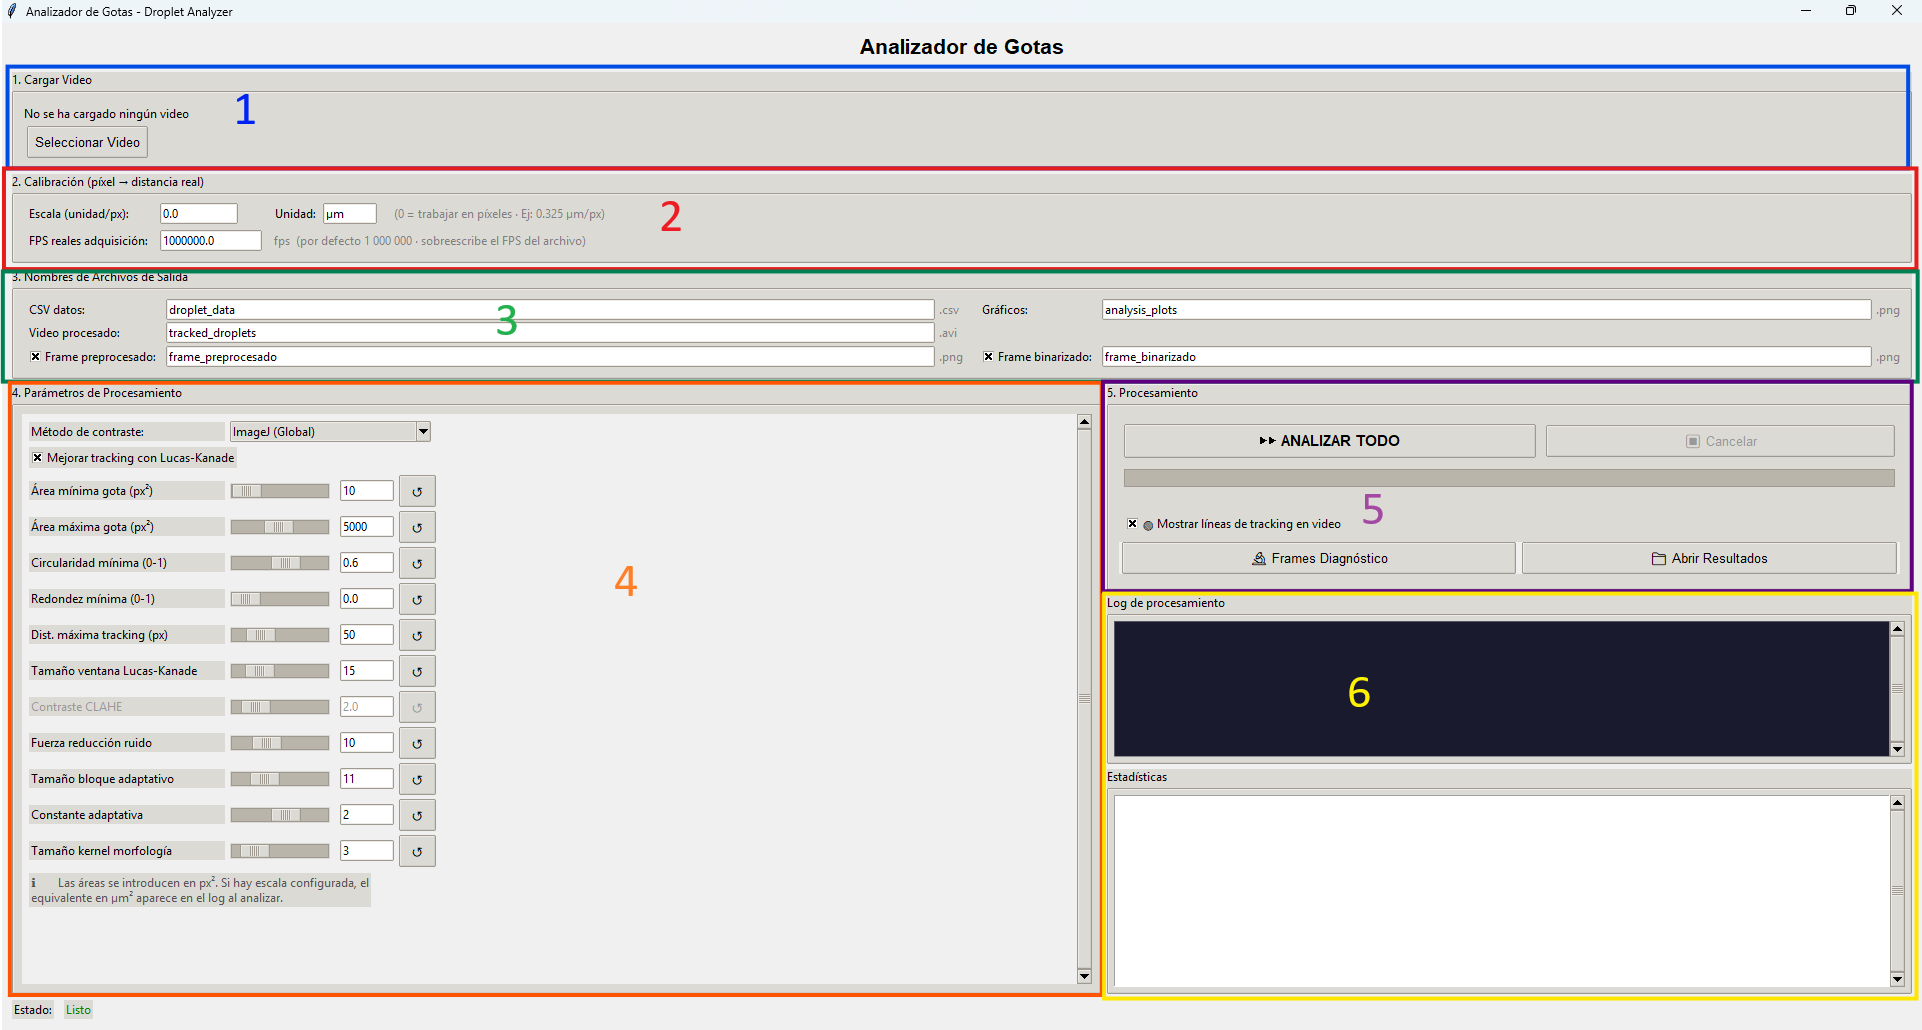
\includegraphics[width=0.9\textwidth]{figures/manual_usuario/desc_interfaz.png}
    \caption{Interfaz gráfica de la aplicación.}
\end{figure}

\section{Procedimiento}

Para analizar un vídeo, el usuario debe seguir los pasos que se detallan en esta sección.

\subsection{Paso 1: Cargar el vídeo}

La carga del vídeo se realiza siguiendo los siguientes pasos en el panel 1:
\begin{enumerate}
    \item Pulsar en el botón \textbf{Seleccionar Vídeo} para abrir el explorador de archivos \ref{fig:cargar_video_a}.
    \item Navegar hasta la ubicación del vídeo a analizar y seleccionarlo \ref{fig:cargar_video_b}.
    \item Una vez cargado, aparecerá el nombre del archivo, los fps y el número de fotogramas \ref{fig:cargar_video_c}.
\end{enumerate}

\begin{figure}[H]
    \centering
    
    \begin{subfigure}[b]{0.5\textwidth}
        \centering
        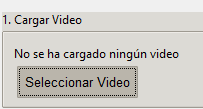
\includegraphics[width=\textwidth]{figures/manual_usuario/CargarVideo1.png}
        \caption{Botón para cargar el vídeo.}
        \label{fig:cargar_video_a}
    \end{subfigure}
    
    \vspace{0.5cm}
    
    \begin{subfigure}[b]{0.6\textwidth}
        \centering
        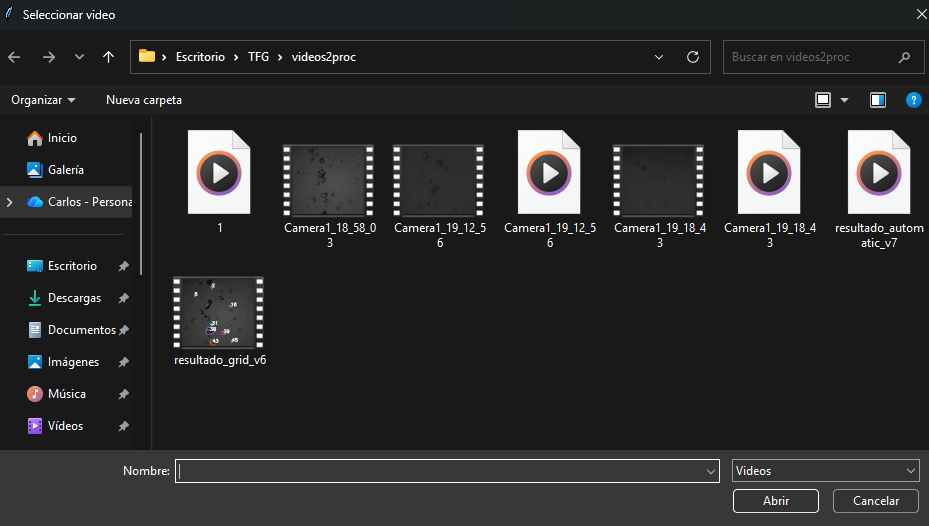
\includegraphics[width=\textwidth]{figures/manual_usuario/CargarVideo2.png}
        \caption{Seleccionar video.}
        \label{fig:cargar_video_b}
    \end{subfigure}

    \vspace{0.5cm}

    \begin{subfigure}[b]{0.5\textwidth}
        \centering
        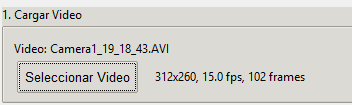
\includegraphics[width=\textwidth]{figures/manual_usuario/CargarVideo3.png}
        \caption{Vídeo cargado.}
        \label{fig:cargar_video_c}
    \end{subfigure}

    \caption{Proceso de carga del vídeo.}
    \label{fig:grupo_total}
\end{figure}

\subsection{Paso 2: Calibración (Escala y FPS)}

Una vez cargado el vídeo, hay que convertir los píxeles a unidades reales y ajustar la tasa de fotogramas reales. Para ello, se deben seguir los siguientes pasos en el panel 2:

\begin{enumerate}
    \item Introducir el factor de conversión de píxeles a unidades reales en el campo \textbf{Escala (unidad/px)}. Si el campo se deja a 0, todos los cálculos se realizarán en píxeles.
    \item Introducir los FPS reales a los que se grabó el vídeo en el campo de entrada \textbf{FPS reales adquisición}. Por defecto toma un valor de $10^{6}$ FPS.
\end{enumerate}

\begin{figure}[H]
    \centering
    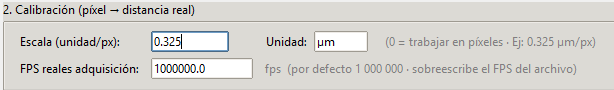
\includegraphics[width=0.8\textwidth]{figures/manual_usuario/Calibracion.png}
    \caption{Panel de calibración.}
\end{figure}

Cabe destacar que el factor de conversión depende del objetivo(zoom) con el que se haya grabado el vídeo, por lo que deberá recalibrarse para cada combinación de zoom y distancia al inyector utilizada en el experimento.

\textbf{Nota:} El campo \textbf{Unidad} es puramente descriptivo y no implica ninguna conversión automática. El usuario debe asegurarse de que el factor numérico introducido sea coherente con la unidad indicada y con el zoom utilizado durante la grabación.

\subsection{Paso 3: Nombres de archivos de salida}

En esta sección (Panel 3) se personalizan los nombres base de todos los ficheros que la
aplicación generará en la carpeta \texttt{output/}. Las extensiones se añaden
automáticamente. Nombres a configurar:
\begin{itemize}
    \item \textbf{Nombre base de CSV datos}: nombre del fichero principal de datos (defecto: droplet\_data.csv).
    \item \textbf{Nombre base de gráficos estadísticos}: nombre del fichero de gráficos estadísticos en PNG (defecto:analysis\_plots.png).
    \item \textbf{Nombre base de vídeo de salida}: nombre del vídeo que se genera con la visualización del procesamiento (defecto: tracked\_droplets.avi).
    \item \textbf{Frame preprocesado}: PNG del primer fotograma tras el preprocesado (activo con el checkbox).
    \item \textbf{Frame binarizado}: PNG del primer fotograma binarizado/segmentado (activo con el checkbox).
\end{itemize}

\begin{figure}[H]
    \centering
    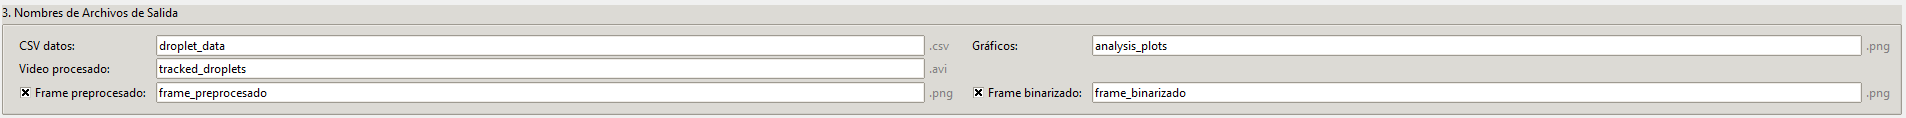
\includegraphics[width=1\textwidth]{figures/manual_usuario/nombres.png}
    \caption{Panel de configuración de nombres de salida.}
\end{figure}

\subsection{Paso 4: Parámetros de procesamiento}
En el panel 4 se configuran todos los parámetros relacionados con el procesamiento de vídeo. Dispone de un selector para elegir entre diferentes procesamientos del histograma, un checbox para activar o desactivar Lucas-Kanade, y varios campos de entrada con sliders para configurar los parámetros numéricos. Para más detalles de los parámetros, consultar la tabla \ref{tab:parametros_gui}.

En la figura \ref{fig:parametros} se muestra el panel de configuración de parámetros. El recuadro A corresponde al botón de reseteo al valor por defecto, el recuadro B al campo de entrada numérico y el recuadro C al slider.

\begin{figure}[H]
    \centering
    \includegraphics[width=0.85\textwidth]{figures/manual_usuario/parametros.png}
    \caption{Panel de configuración de parámetros de procesamiento.}
    \label{fig:parametros}
\end{figure}

\subsection{Paso 5: Procesamiento}

La ejecución del procesamiento se controla desde el panel 5. Para iniciar el procesamiento hay que pulsar el botón \textbf{Analizar Todo}. Esto analizará el vídeo completo, generando todos lo archivos de salida en la carpeta \texttt{output/}.
Antes de lanzar el procesamiento, podemos desactivar el checkbox \textbf{Mostrar líneas de tracking de vídeo} para que en el vídeo de salida no se pinten las trazas del seguimiento de las gotas.
Durante el procesamiento, la barra de progreso se va actualizando para mostrar el avance. El log de procesamiento (Panel 6) nos mostrará en tiempo real logs del procesamiento.

Si pulsamos el botón \texttt{Cancelar} se detendrá el análisis en el siguiente fotograma sin generar los archivos de salida.

\begin{figure}[H]
    \centering
    \includegraphics[width=0.9\textwidth]{figures/manual_usuario/procesamiento1.png}
    \caption{Panel de control de procesamiento.}
    \label{fig:procesamiento}
\end{figure}

Durante el procesamiento se abre una ventana flotante para previsualizar el análisis en tiempo real. Se muestra el fotograma original, el preprocesado, el binrizado y el final con las gotas detectadas y las líneas de tracking (si el checkbox está activo).

\begin{figure}[H]
    \centering
    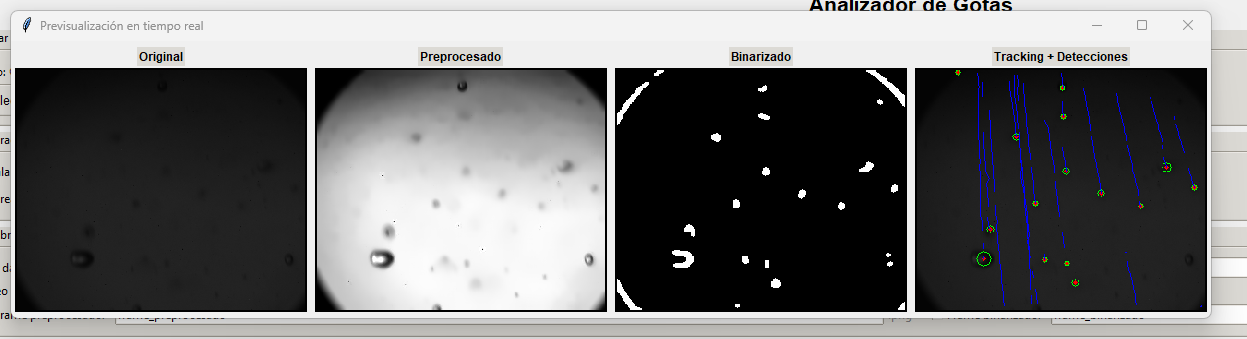
\includegraphics[width=0.9\textwidth]{figures/manual_usuario/previsualizacion.png}
    \caption{Ventana de previsualización en tiempo real.}
    \label{fig:previsualizacion}
\end{figure}

Una vez finalizado el procesamiento, aparecerán las estadísticas generales en la sección de log (Panel 6). Si pulsamos el botón \textbf{Abrir resultados} se abrirá la carpeta \texttt{output/} en el explorador de archivos.

\begin{figure}[H]
    \centering
    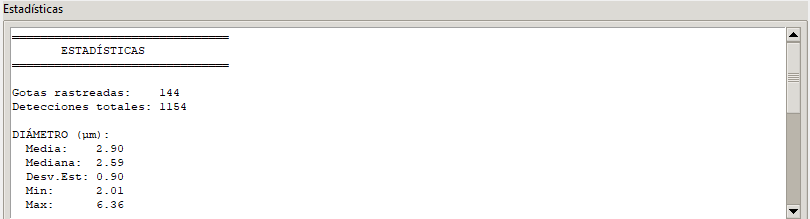
\includegraphics[width=0.9\textwidth]{figures/manual_usuario/estadisticas.png}
    \caption{Sección de estadísticas.}
    \label{fig:estadisticas}
\end{figure}

\section{Flujo recomendado para el ajuste de parámetros}

Para ajustar los parámetros de manera eficiente, sin lanzar el análisis completo cada vez, se recomienda seguir el siguiente flujo de trabajo:
\begin{enumerate}
    \shorthandoff{"}
    \item Cargue el vídeo y haga clic en "Frames Diagnóstico" sin cambiar ningún parámetro.
    \item Observe el frame binarizado. Si hay demasiado ruido, aumente  "Fuerza reducción" ruido o "Tamaño kernel morfología".
    \item Si las gotas no se detectan (aparecen en negro), ajuste "Constante adaptativa" o "Tamaño bloque adaptativo".
    \item Filtre por tamaño usando "Área mínima" y "Área máxima" para excluir artefactos.
    \item Ajuste "Circularidad mínima" o "Redondez mínima" según la forma real de sus gotas.
    \item Una vez satisfecho con la segmentación, lance el análisis completo.
\end{enumerate}

\section{Archivos de salida}

Al terminar el análisis se generan en la carpeta \texttt{output/} los siguientes archivos con información útil:

\begin{itemize}
    \item \textbf{CSV general}: Contiene información de las diferentes medidas por frame y track\_id.
    \item \textbf{Video de salida}: Contiene el vídeo procesado con las gotas detectadas y las líneas de tracking.
    \item \textbf{CSVs individuales}: Varios archivos CSV con la información de los ejes de las gráficas generadas.
    \item \textbf{Gráficas}: Archivos de imagen con las gráficas generadas a partir de los datos procesados.
    \item \textbf{Frames de diagnóstico}: Imagenes PNG del primer frame tras aplicar el preprocesado y la binarización.
\end{itemize}

En la figura \ref{fig:graficas} se muestra un ejemplo de las gráficas generadas a partir de los datos procesados. Estas gráficas incluyen información sobre la distribución de tamaños de gotas, velocidades, trayectorias, entre otras métricas relevantes para el análisis de las gotas.

\begin{figure}[H]
    \centering
    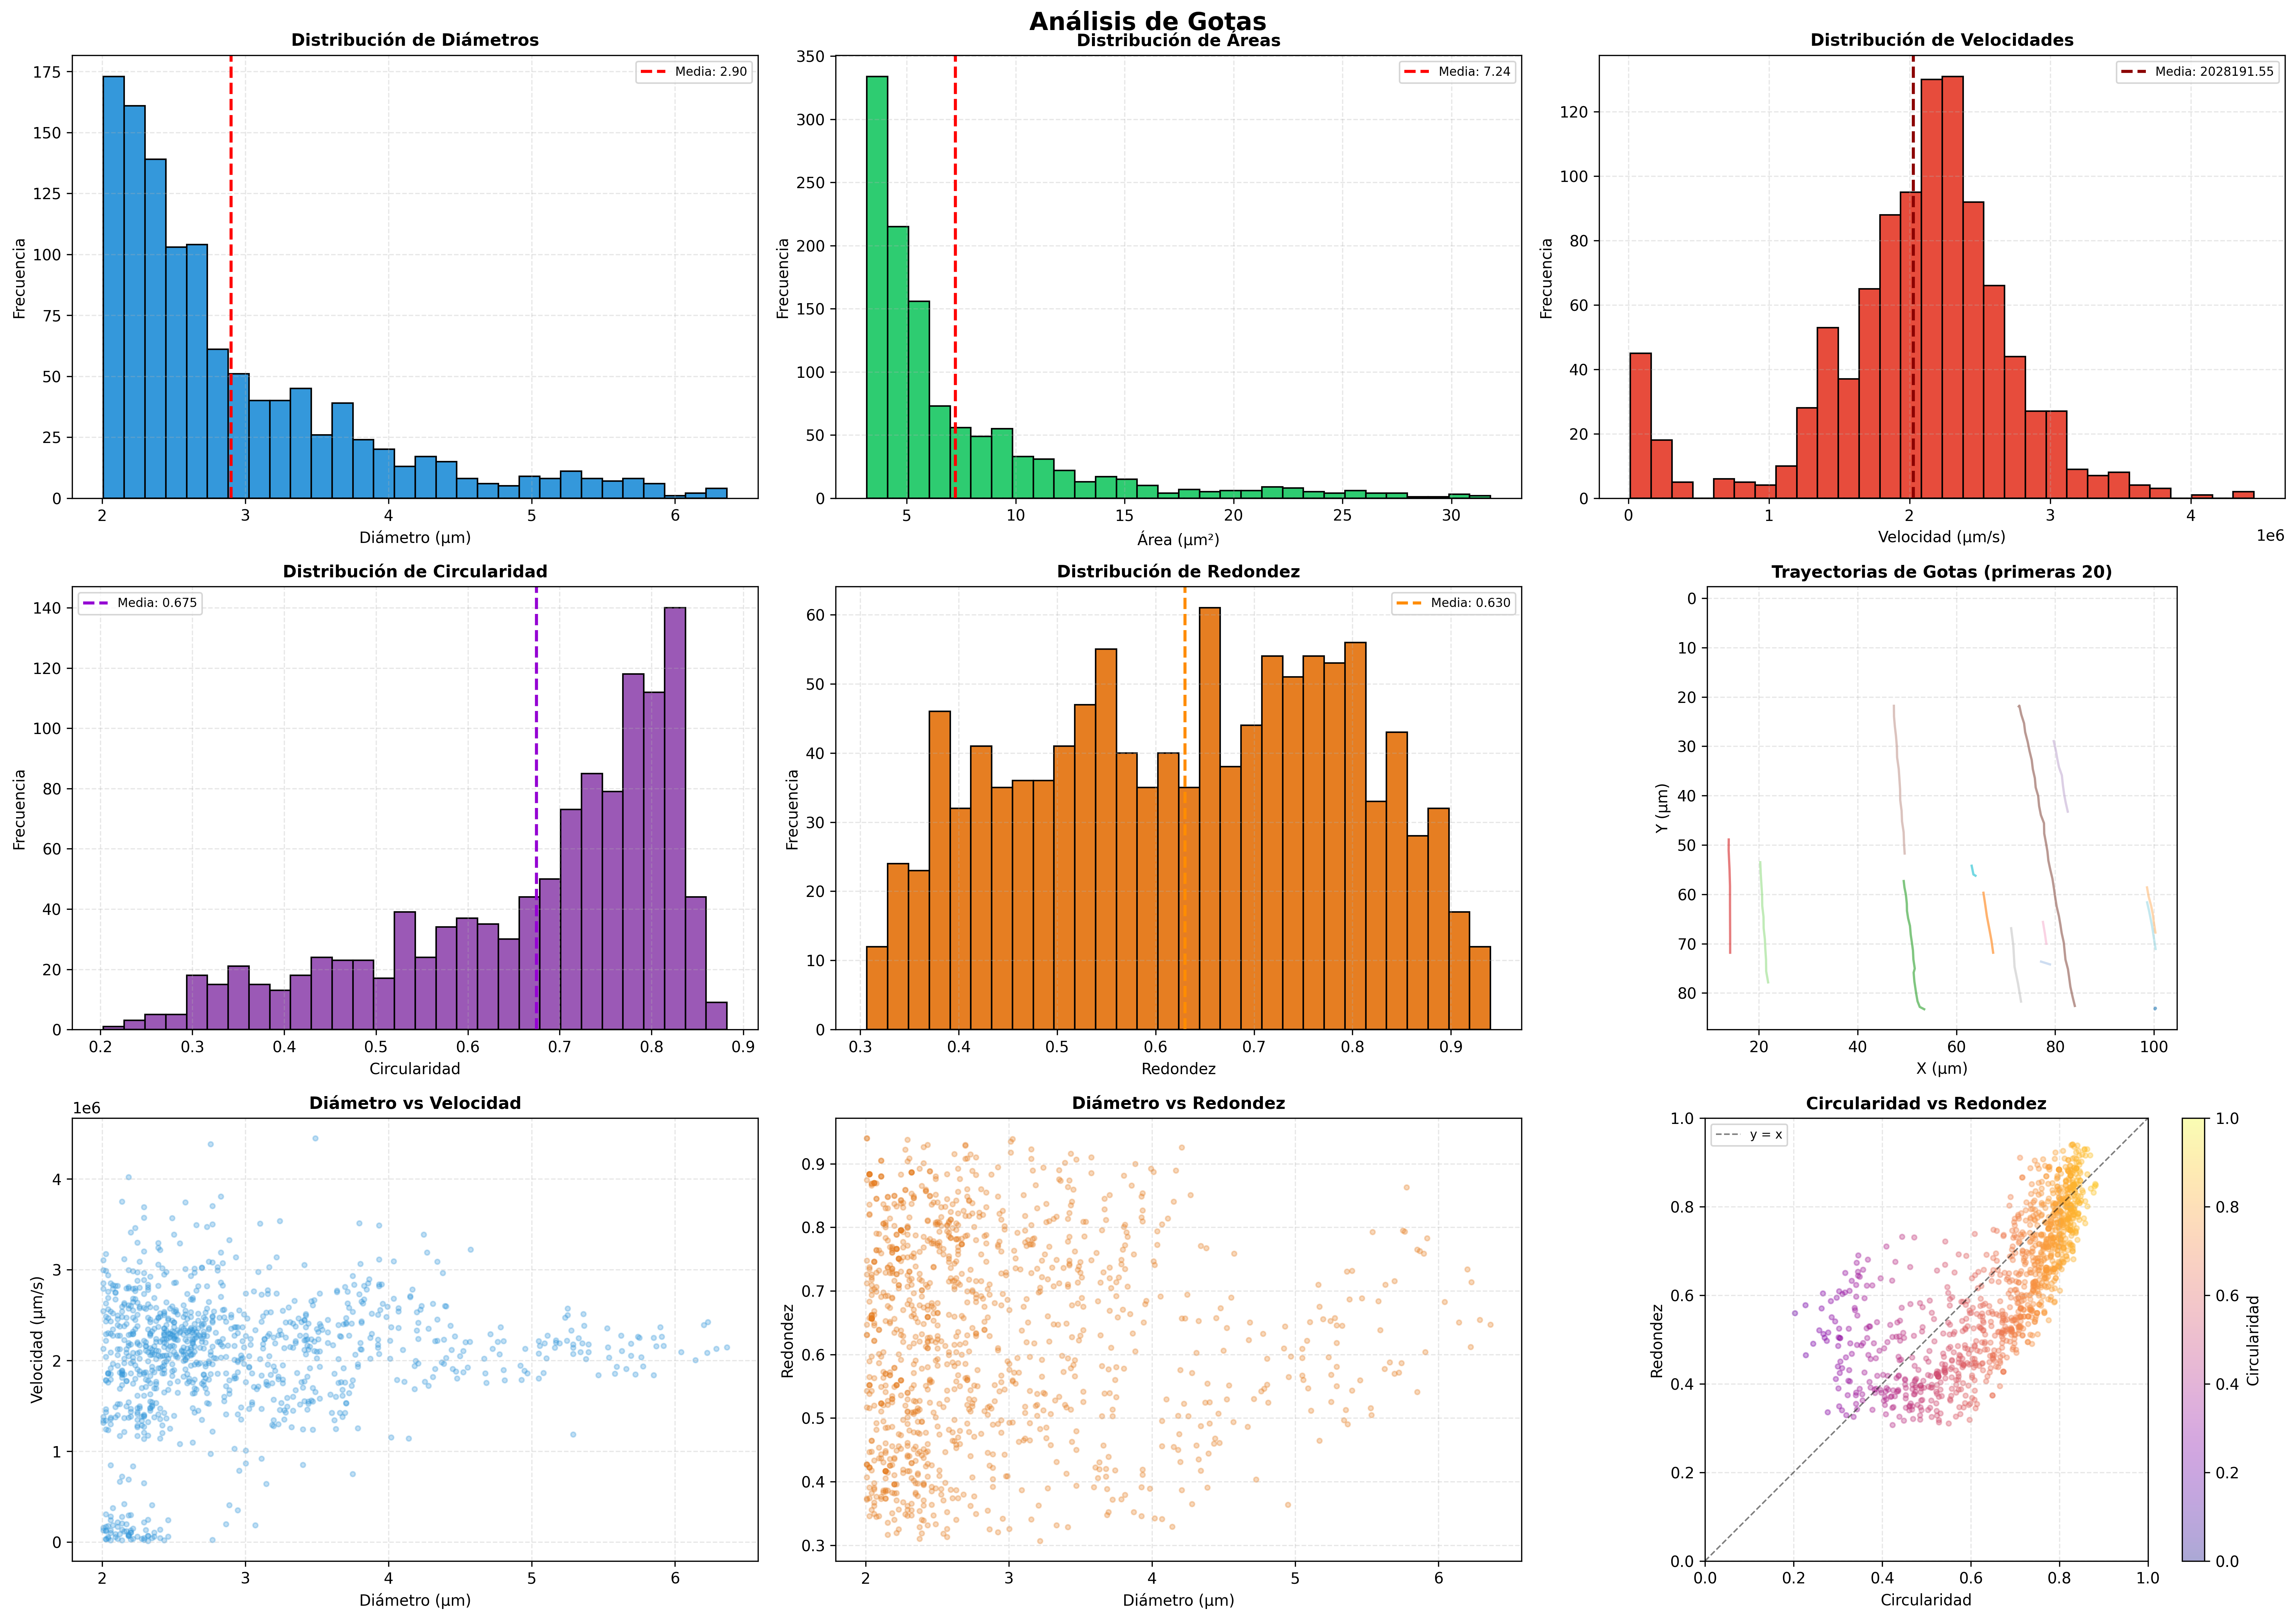
\includegraphics[width=1\textwidth]{figures/manual_usuario/analysis_plots.png}
    \caption{Ejemplo de las gráficas generadas.}
    \label{fig:graficas}
\end{figure}

    % LTeX: language=es

\chapter{Resultados y Evaluación} \label{chap:resultados}

En este capítulo se presentan los resultados del analizador implementado. La evaluación se ha dividido en dos partes complementarias: una evaluación \textbf{cualitativa}, en la que se analiza el desempeño de la aplicación sobre vídeos reales de experimentos; y una evaluación \textbf{cuantitativa}, en la que se analiza el error cometido por el analizador con respecto al ground truth de un conjunto de vídeos generados sintéticamente.

\section{Metodología de Evaluación}

Evaluar una aplicación de visión por computador requiere disponer de una referencia con la que comparar las mediciones. En experimentos reales esto es difícil, ya que no se conoce con exactitud el diámetro o velocidad de las gotas. Para solucionar este problema, se han generado vídeos de gotas con características conocidas (ground truth), mediante una serie de scripts de evaluación desarrollados en Python.

\subsection{Scripts de evaluación}

El sistema de evaluación consta de tres scripts independientes capaces de ejecutar los experimentos de forma autónoma:

\begin{itemize}
     \item \texttt{synthetic\_video\_generator.py}: Genera los vídeos sintéticos con gotas y los ficheros CSV de ground truth. Cada gota se dibuja como un disco blanco con borde gaussiano suavizado sobre un fondo oscuro, con posición, velocidad y diámetro exactamente conocidos. Se admite la adición de ruido gaussiano y de tipo sal y pimienta de intensidad configurable. El script expone una función por experimento (\texttt{experiment\_E1\_segmentation}, \texttt{experiment\_E2\_velocity}, etc.) y puede ejecutarse directamente desde la línea de comandos indicando los experimentos deseados. Este script también se encarga de generar los ficheros CSV de ground truth, con la siguiente información: \texttt{frame}, \texttt{track\_id}, \texttt{x\_px}, \texttt{y\_px}, \texttt{diameter\_px}, \texttt{vx\_px\_frame} y \texttt{vy\_px\_frame}.
     \item \texttt{run\_experiments.py}: Ejecuta el pipeline completo de análisis. Para cada subexperimento genera los vídeos sintéticos llamando a \texttt{synthetic\_video\_generator.py}, luego se conecta directamente al backend del analizador para procesar el vídeo generado, por último compara los resultados obtenidos con el groundtruth mediante \texttt{DropletEvaluator}. Este script puede lanzar todos los experimentos o un subconjunto en particular con el argumento \texttt{--experiments}.
    \item \texttt{plot\_experiment.py}: Genera las gráficas de resultados para un único experimento a partir de su CSV de métricas. Su uso se muestra en el listing \ref{lst:plot_experiment}.
\end{itemize}

\begin{lstlisting}[language=bash, caption={Uso del script de generación de gráficas por experimento.}, label={lst:plot_experiment}]
#Generar las gráficas para el experimento E1.
python plot_experiment.py E1 --metrics_csv results/E1_metrics.csv

#Generar las gráficas para el experimento E4 con mayor resolución.
python plot_experiment.py E4 --metrics_csv results/E4_metrics.csv --dpi 300 --show
\end{lstlisting}

\subsection{Métricas de evaluación}

El evaluador calcula las siguientes métricas \cite{powers2011evaluation}\cite{everingham2010pascal} para cada vídeo analizado. El emparejamiento entre detecciones y gotas GT se realiza por distancia euclídea mínima entre centroides, con un umbral máximo de 15px:

\begin{itemize}
    \item \textbf{Precisión, Recall y F1:} Miden la tasa de detecciones correctas respecto al total de gotas presentes (GT) y al total de detecciones realizadas. Una detección se considera correcta si su centroide se encuentra a menos de 15~px del centroide GT más cercano.
    \item \textbf{MRE\textsubscript{diam}:} Error Relativo Medio del diámetro, definido como $\text{MRE} = \frac{1}{N}\sum_{i=1}^{N}\frac{|d_i^{\text{det}} - d_i^{\text{GT}}|}{d_i^{\text{GT}}}$.
    \item \textbf{RMSE\textsubscript{diam}:} Raíz del Error Cuadrático Medio del diámetro en píxeles.
    \item \textbf{Circularidad media:} Media y desviación estándar de la circularidad detectada, que en gotas sintéticas perfectamente circulares debería ser próxima a 1.
    \item \textbf{MRE\textsubscript{vel} y RMSE\textsubscript{vel}:} Error relativo y RMSE de la magnitud de velocidad detectada respecto a la velocidad GT.
    \item \textbf{Tasa de fragmentación:} Definida como $\frac{N_{\text{tracks det}} - N_{\text{tracks GT}}}{N_{\text{tracks GT}}}$, indica si el tracker divide una única trayectoria real en varios tracks.
\end{itemize}

\subsection{Evaluación cuantitativa}

\subsection{E1 - Precisión de segmentación con diámetros conocidos}
 
\textbf{Configuración:} Se generaron vídeos de 30 frames con 4 gotas estáticas por frame en cuadrícula, sin ruido, para 7 diámetros distintos: 6, 10, 15, 20, 30, 40 y 50~px. Al ser gotas estáticas e idealmente circulares, este experimento aísla el error puro de la etapa de segmentación y medición, sin la influencia del tracking ni del ruido.

En la figura \ref{fig:E1} se muestra un frame del vídeo generado para este experimento.
\begin{figure}[H]
    \centering
    
\includegraphics[width=0.4\textwidth]{figures/E1.png}
    \caption{Frame de uno de los vídeos generado para E1.}
    \label{fig:E1}
\end{figure}


\begin{table}[H]
\centering
\small
\caption{Resultados del experimento E1 (precisión de segmentación).}
\begin{tabular}{ccccccc}
\hline
\textbf{Diámetro GT (px)} & \textbf{Recall} & \textbf{Precision} & \textbf{F1} & \textbf{MRE\textsubscript{diam} (\%)} & \textbf{RMSE\textsubscript{diam} (px)} & \textbf{Circ. media} \\
\hline
6  & 1.00 & 1.00 & 1.00 & 62.32 & 3.74 & 0.8612 \\
10 & 1.00 & 1.00 & 1.00 & 39.12 & 3.91 & 0.8786 \\
15 & 1.00 & 1.00 & 1.00 & 23.72 & 3.56 & 0.9003 \\
20 & 1.00 & 1.00 & 1.00 & 19.19 & 3.84 & 0.8774 \\
30 & 1.00 & 1.00 & 1.00 & 12.93 & 3.88 & 0.8579 \\
40 & 1.00 & 1.00 & 1.00 & 9.64  & 3.86 & 0.8962 \\
50 & 1.00 & 1.00 & 1.00 & 7.73  & 3.87 & 0.8793 \\
\hline
\end{tabular}
\label{tab:e1_resultados}
\end{table}

Como se pueden observar en los resultados mostrados en la tabla \ref{tab:e1_resultados} y en la figura \ref{fig:E1_metrics}, el analizador detecta correctamente todas las gotas (Recall y Precision de 1.00) para todos los diámetros, lo que indica que la segmentación es robusta incluso para gotas pequeñas. Sin embargo, se observa un error absoluto constante en la segmentación de aproximadamente 3.8 píxeles, debido a la discretización digital y umbralización, que también explica por qué la métrica de circularidad se penaliza por el efecto escalera de los bordes perimetrales mientras que la redondez se mantiene excelente por encima de 0.95. Aunque este ensanchamiento sistemático del contorno es prácticamente despreciable en gotas grandes (reduciendo el error relativo al 7.7\% en diámetros de 50 px), resulta un factor crítico al evaluar las microgotas de 6 px, cuyo tamaño se sobreestima en más de un 62\%.

\begin{figure}[htbp]
    \centering
        
    \begin{subfigure}[b]{0.7\textwidth}
        \centering
        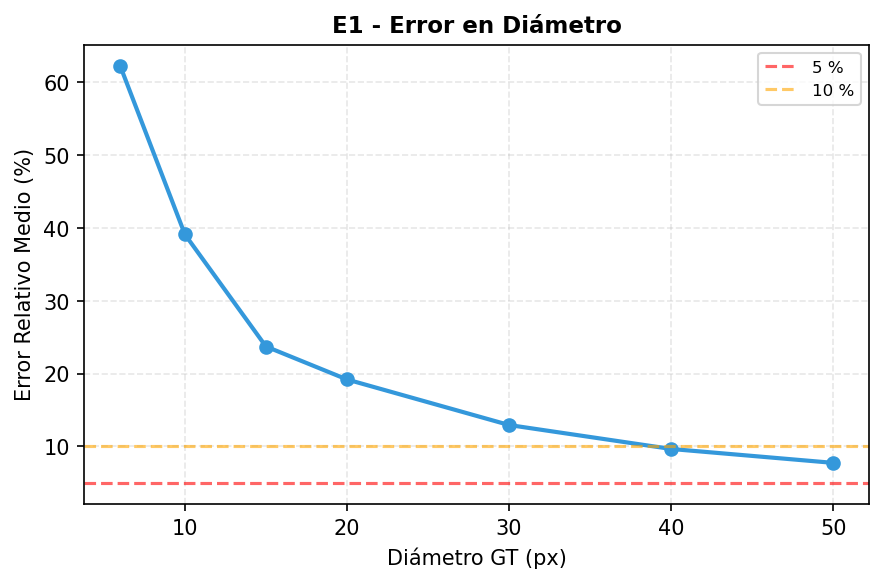
\includegraphics[width=\textwidth]{figures/tests/E1/E1_mre_diam.png}
    \end{subfigure}
    \begin{subfigure}[b]{0.7\textwidth}
        \centering
        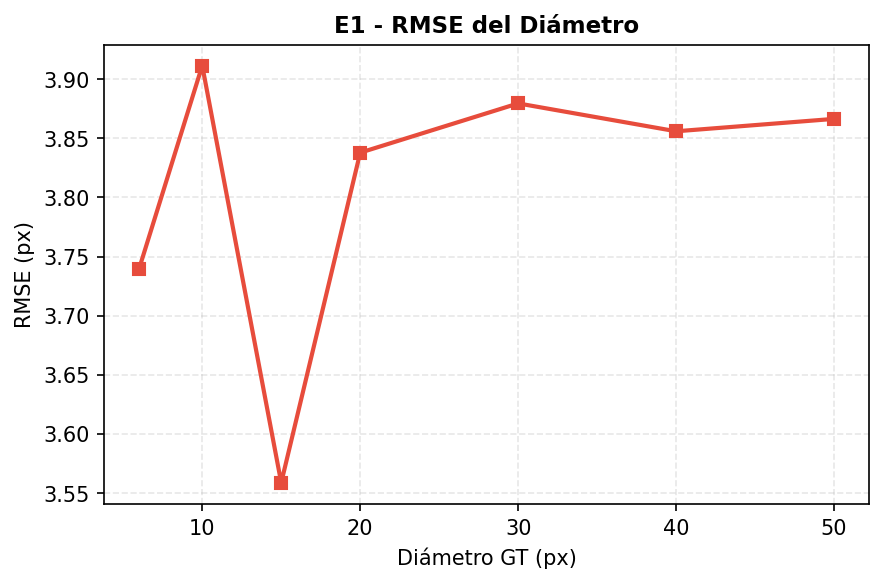
\includegraphics[width=\textwidth]{figures/tests/E1/E1_rmse_diam.png}
    \end{subfigure}
    \begin{subfigure}[b]{0.7\textwidth} 
        \centering
        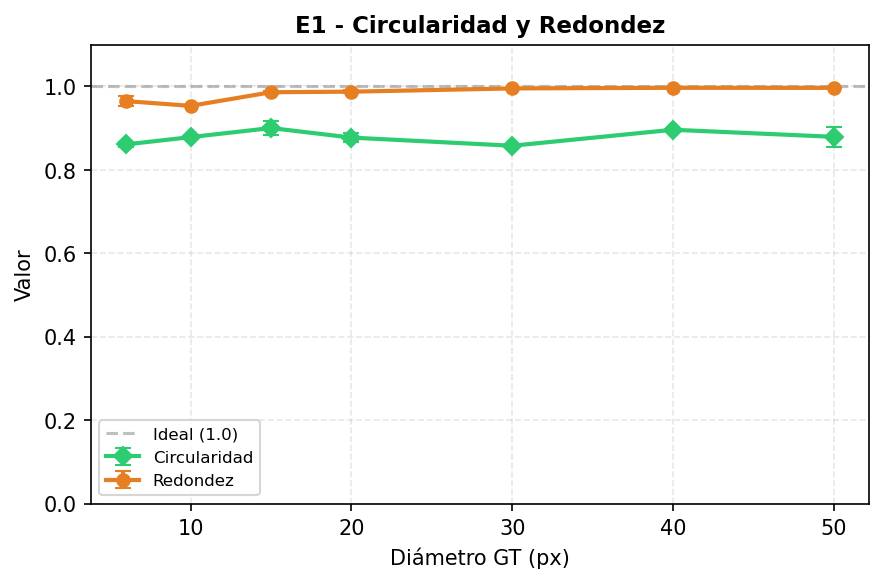
\includegraphics[width=\textwidth]{figures/tests/E1/E1_shape_metrics.png}
    \end{subfigure}
    
    \caption{Métricas de error de diámetro y forma para el experimento E1.}
    \label{fig:E1_metrics}
\end{figure}

\subsection{E2 - Precisión en la estimación de velocidad}
 
\textbf{Configuración:} Se generaron 5 vídeos de 60 frames con una única gota de 20~px de diámetro moviéndose a velocidad constante y conocida, cubriendo movimientos horizontal, vertical y diagonal en ambos sentidos, con magnitudes entre 2 y $\sqrt{4^2+2^2} \approx 4.5$~px/frame. La velocidad real de los experimentos de nebulización es del orden de miles de µm/ms, lo que a la escala del vídeo y con la tasa de adquisición usada equivale a pocos píxeles por frame; este rango es, por tanto, representativo.

\begin{table}[H]
\centering
\small
\caption{Resultados del experimento E2 (precisión de la estimación de velocidad y tracking). La velocidad se expresa en píxeles por frame (px/f).}
\begin{tabular}{ccccccc}
\hline
\textbf{($v_x, v_y$)} & \textbf{Velocidad GT} & \textbf{Velocidad Det.} & \textbf{MRE\textsubscript{vel} (\%)} & \textbf{RMSE\textsubscript{vel}} & \textbf{F1 Track} & \textbf{Frag.} \\
\hline
(2.0, 0.0)  & 2.000 px/f & 2.001 $\pm$ 0.018 px/f & 0.44 & 0.0090 px/f & 1.0 & 0.0 \\
(5.0, 0.0)  & 5.000 px/f & 5.001 $\pm$ 0.015 px/f & 0.12 & 0.0029 px/f & 1.0 & 0.0 \\
(0.0, 3.0)  & 3.000 px/f & 3.001 $\pm$ 0.014 px/f & 0.19 & 0.0045 px/f & 1.0 & 0.0 \\
(3.0, 3.0)  & 4.243 px/f & 4.244 $\pm$ 0.038 px/f & 0.45 & 0.0088 px/f & 1.0 & 0.0 \\
(-4.0, 2.0) & 4.472 px/f & 4.472 $\pm$ 0.013 px/f & 0.17 & 0.0029 px/f & 1.0 & 0.0 \\
\hline
\end{tabular}
\label{tab:e2_resultados}
\end{table}
 

\begin{figure}[htbp]
    \centering
        
    \begin{subfigure}[b]{0.85\textwidth}
        \centering
        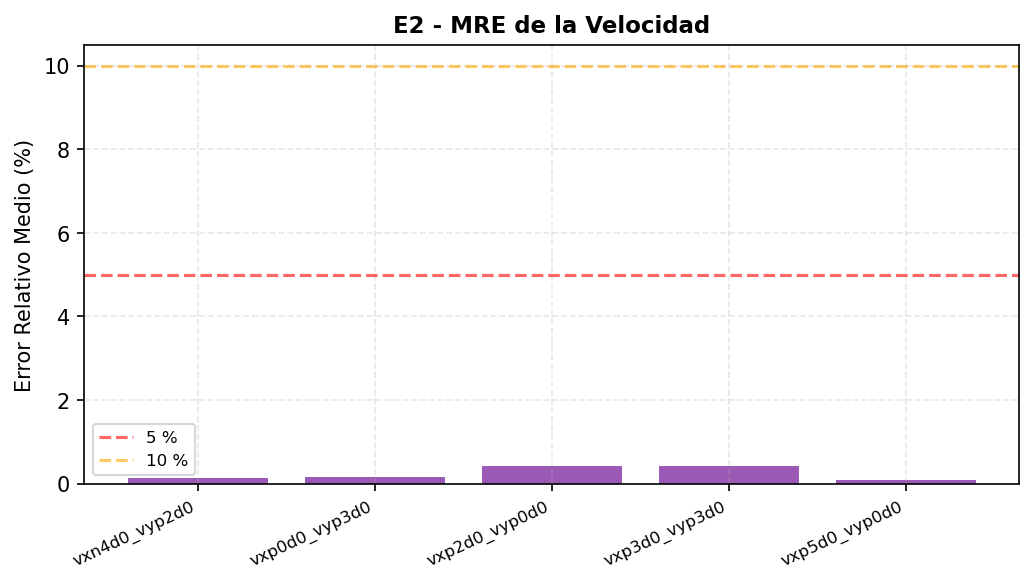
\includegraphics[width=\textwidth]{figures/tests/E2/E2_mre_vel.png}
    \end{subfigure}
    \begin{subfigure}[b]{0.85\textwidth}
        \centering
        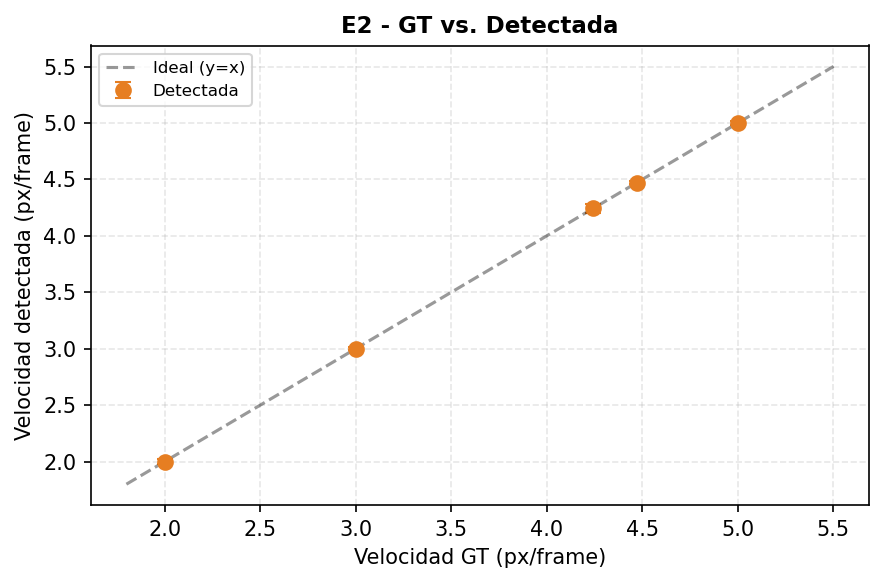
\includegraphics[width=\textwidth]{figures/tests/E2/E2_gt_vs_det.png}
    \end{subfigure}

    \caption{Métricas de error de velocidad para el experimento E2.}
    \label{fig:E2_metrics}
\end{figure}

En los datos mostrados en la tabla \ref{tab:e2_resultados} y en la figura \ref{fig:E2_metrics}, se aprecia que el analizador detecta la trayectoria completa y sin fragmentación (F1 de tracking de 1.0 y tasa de fragmentación de 0.0) en todos los casos. Por otro lado, el error relativo medio en la velocidad estimada es inferior al 0.5\% en todos los casos. Todo esto demuestra el excelente desempeño del analizador bajo condiciones sin ruido y con gota de tamaño moderado.


\subsection{E3 - Robustez al ruido}
 
\textbf{Configuración:} Se usó una única gota estática de 20~px de diámetro, evaluada bajo dos tipos de degradación de forma independiente: (a) ruido gaussiano aditivo con $\sigma \in \{0, 5, 10, 20, 35, 50\}$ y (b) ruido de tipo sal y pimienta con fracción de píxeles afectados $\in \{0\%, 2\%, 5\%, 10\%\}$. Este experimento permite caracterizar la sensibilidad del pipeline de preprocesamiento y segmentación ante condiciones de imagen degradada, habituales en los vídeos de alta velocidad donde la limitación de luz provoca un mayor nivel de ruido electrónico en el sensor.

\begin{figure}[H]
    \centering
    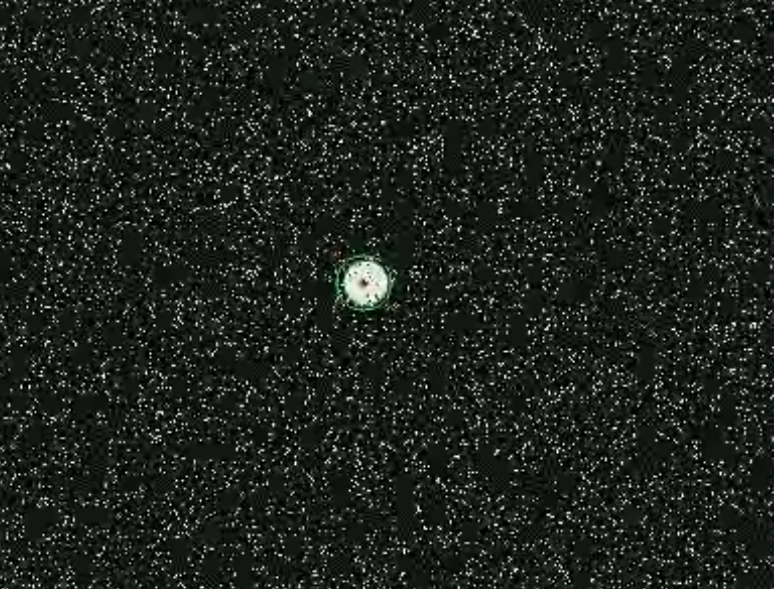
\includegraphics[width=0.4\textwidth]{figures/E3.png}
    \caption{Ejemplo de degradación por sal y pimienta al 10\%}
\end{figure}

\begin{table}[H]
\centering
\small
\caption{Resultados del experimento E3 (robustez al ruido gaussiano y sal y pimienta en gotas de 20 px).}
\begin{tabular}{lrccccc}
\hline
\textbf{Tipo de Ruido} & \textbf{Nivel} & \textbf{Recall} & \textbf{F1} & \textbf{MRE\textsubscript{diam} (\%)} & \textbf{RMSE\textsubscript{diam} (px)} & \textbf{Circ. media} \\
\hline
\multicolumn{7}{c}{\textit{Ruido Gaussiano ($\sigma$)}} \\
\hline
Gaussiano & 0  & 1.00 & 1.00 & 43.06 & 8.61 & 0.9291 \\
Gaussiano & 5  & 1.00 & 1.00 & 43.25 & 8.65 & 0.8766 \\
Gaussiano & 10 & 1.00 & 1.00 & 44.54 & 8.91 & 0.8284 \\
Gaussiano & 20 & 1.00 & 1.00 & 45.79 & 9.16 & 0.7900 \\
Gaussiano & 35 & 1.00 & 1.00 & 46.14 & 9.23 & 0.6930 \\
Gaussiano & 50 & 0.98 & 0.99 & 45.85 & 9.17 & 0.5526 \\
\hline
\multicolumn{7}{c}{\textit{Ruido Sal y Pimienta}} \\
\hline
Sal y Pimienta & 0\%  & 1.00 & 1.00 & 43.06 & 8.61 & 0.9291 \\
Sal y Pimienta & 2\%  & 1.00 & 1.00 & 43.50 & 8.70 & 0.8545 \\
Sal y Pimienta & 5\%  & 1.00 & 1.00 & 44.55 & 8.91 & 0.7652 \\
Sal y Pimienta & 10\% & 0.95 & 0.97 & 44.34 & 8.87 & 0.6100 \\
\hline
\end{tabular}
\label{tab:e3_resultados}
\end{table}

Como compromiso de diseño, se ha priorizado la detección y localización de las gotas por encima de la precisión de su diámetro. Esta severa reducción de ruido distorsiona y erosiona los contornos originales, provocando una pérdida de píxeles que infla el error absoluto del diámetro medido (RMSE\textsubscript{diam} $\approx$ 8.6 - 9.2 px) y deteriora de forma progresiva la métrica de circularidad debido a la irregularidad de los bordes resultantes. Sin embargo, esta estrategia asegura el éxito del tracking: la métrica F1 se mantiene excepcionalmente robusta y muy por encima del 90\% (superando el 97\% incluso en los escenarios críticos de $\sigma=50$ y $10\%$ de píxeles corruptos). Cabe destacar que se podría haber optado por una configuración de filtrado menos conservadora para mantener un diámetro más preciso; no obstante, dicha alternativa habría implicado perder la pista de numerosas gotas enmascaradas por el ruido (falsos negativos), hundiendo la tasa de recuperación (Recall) y comprometiendo el análisis de trayectorias.

\begin{figure}[H]
    \centering
        
    \begin{subfigure}[b]{0.7\textwidth}
        \centering
        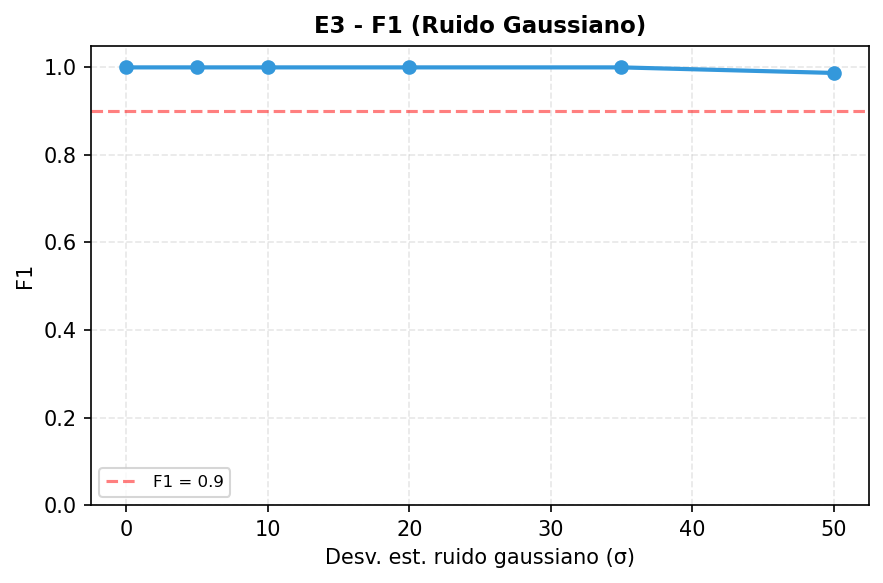
\includegraphics[width=\textwidth]{figures/tests/E3/E3_gauss_f1.png}
    \end{subfigure}
    \begin{subfigure}[b]{0.7\textwidth}
        \centering
        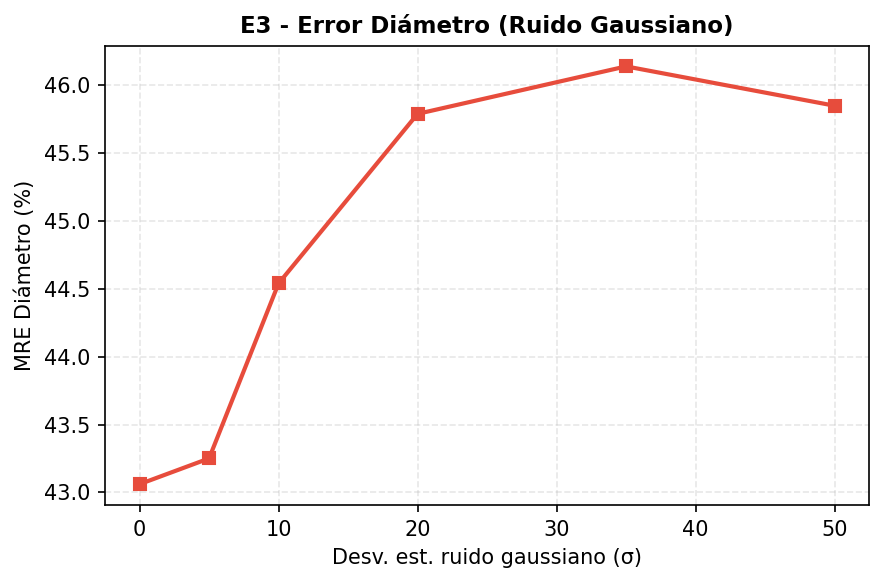
\includegraphics[width=\textwidth]{figures/tests/E3/E3_gauss_mre.png}
    \end{subfigure}

    \caption{Métricas de robustez al ruido gaussiano para el experimento E3.}
    \label{fig:E3_metrics_gauss}
\end{figure}

\begin{figure}[H]
    \centering
        
    \begin{subfigure}[b]{0.7\textwidth}
        \centering
        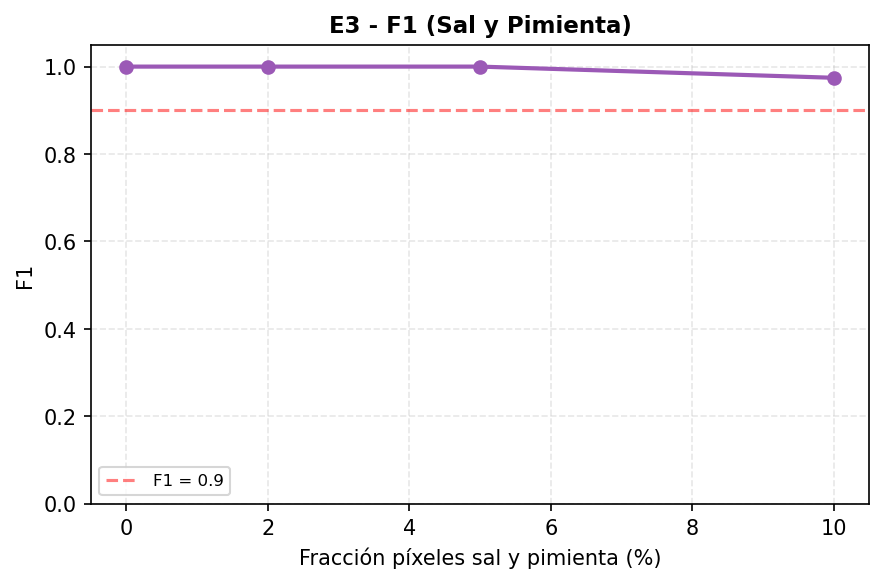
\includegraphics[width=\textwidth]{figures/tests/E3/E3_sp_f1.png}
    \end{subfigure}
    \begin{subfigure}[b]{0.7\textwidth}
        \centering
        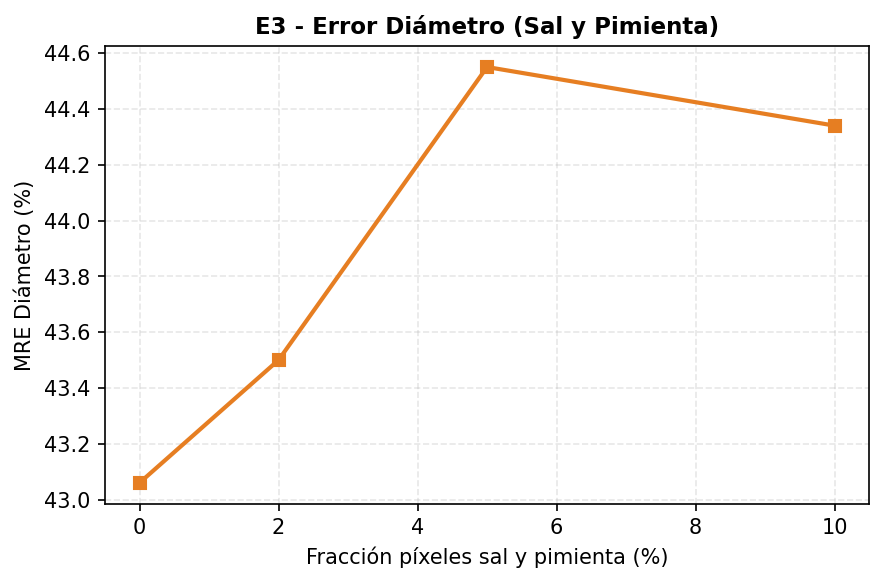
\includegraphics[width=\textwidth]{figures/tests/E3/E3_sp_mre.png}
    \end{subfigure}

    \caption{Métricas de robustez al ruido de tipo sal y pimienta para el experimento E3.}
    \label{fig:E3_metrics_sp}
\end{figure}

\subsection{E4 - Rango de tamaños detectables}
 
\textbf{Configuración:} Se generó un vídeo por cada diámetro del barrido $\{3, 4, 5, 6, 8, 10, 12, 15, 20, 25, 30, 40, 50, 60, 70, 80\}$~px, con una única gota centrada en el frame y ruido gaussiano de $\sigma = 8$ para simular condiciones realistas. Este experimento permite determinar el \textbf{límite inferior} de detección (diámetro mínimo fiable) y el \textbf{límite superior} (a partir del cual el área supera el umbral máximo configurado).

\begin{table}[H]
\centering
\small
\caption{Resultados del experimento E4 (Rango de tamaños detectables). Se omitió la columna Precision porque mantuvo un valor constante de 1.0 en todos los escenarios.}
\begin{tabular}{cccccc}
\hline
\textbf{Diámetro GT (px)} & \textbf{Recall} & \textbf{F1} & \textbf{MRE\textsubscript{diam} (\%)} & \textbf{RMSE\textsubscript{diam} (px)} & \textbf{Circ. media} \\
\hline
3  & 0.80 & 0.89 & 178.95 & 5.38 & 0.7134 \\
4  & 0.93 & 0.97 & 135.23 & 5.42 & 0.7291 \\
5  & 0.97 & 0.98 & 107.95 & 5.40 & 0.6876 \\
6  & 0.97 & 0.98 & 91.45  & 5.49 & 0.6943 \\
8  & 0.97 & 0.98 & 68.41  & 5.48 & 0.6870 \\
10 & 0.90 & 0.95 & 54.46  & 5.45 & 0.6736 \\
12 & 0.97 & 0.98 & 45.01  & 5.40 & 0.7042 \\
15 & 0.97 & 0.98 & 36.69  & 5.51 & 0.6830 \\
20 & 1.00 & 1.00 & 27.83  & 5.57 & 0.7238 \\
25 & 1.00 & 1.00 & 22.21  & 5.55 & 0.7360 \\
30 & 1.00 & 1.00 & 18.55  & 5.57 & 0.7847 \\
40 & 1.00 & 1.00 & 14.15  & 5.66 & 0.7949 \\
50 & 1.00 & 1.00 & 11.22  & 5.61 & 0.8282 \\
60 & 1.00 & 1.00 & 9.24   & 5.55 & 0.8356 \\
70 & 1.00 & 1.00 & 7.84   & 5.49 & 0.8389 \\
80 & 1.00 & 1.00 & 6.99   & 5.60 & 0.8376 \\
\hline
\end{tabular}
\label{tab:e4_resultados}
\end{table}

El sistema demuestra una excelente capacidad de localización incluso en el límite inferior. La métrica Recall supera el umbral de viabilidad (0.80) desde las gotas más diminutas de 3 px, y alcanza una recuperación perfecta (Recall = 1.0 y F1 = 1.0) de forma sostenida a partir de los 20 px. Al igual que en los experimentos anteriores, la precisión de la detección de presencia de gotas se desvincula de la fidelidad geométrica: el algoritmo presenta un ensanchamiento perimetral constante evidenciado por un error absoluto altamente estable (RMSE\textsubscript{diam} $\approx$ 5.5 px). Como se aprecia claramente en el gráfico del error de medición \ref{fig:E4_metrics}, este sesgo sistemático provoca una degradación del MRE\textsubscript{diam}, limitando la precisión para las gotas inferiores a 20 px. No obstante, para gotas medianas y grandes, el error relativo cae rápidamente por debajo de la cota del 10\%, validando el método para conteo en todo el espectro de tamaños y ofreciendo mediciones geométricas fiables para las gotas de un tamaño medio.

\begin{figure}[H]
    \centering
        
    \begin{subfigure}[b]{0.85\textwidth}
        \centering
        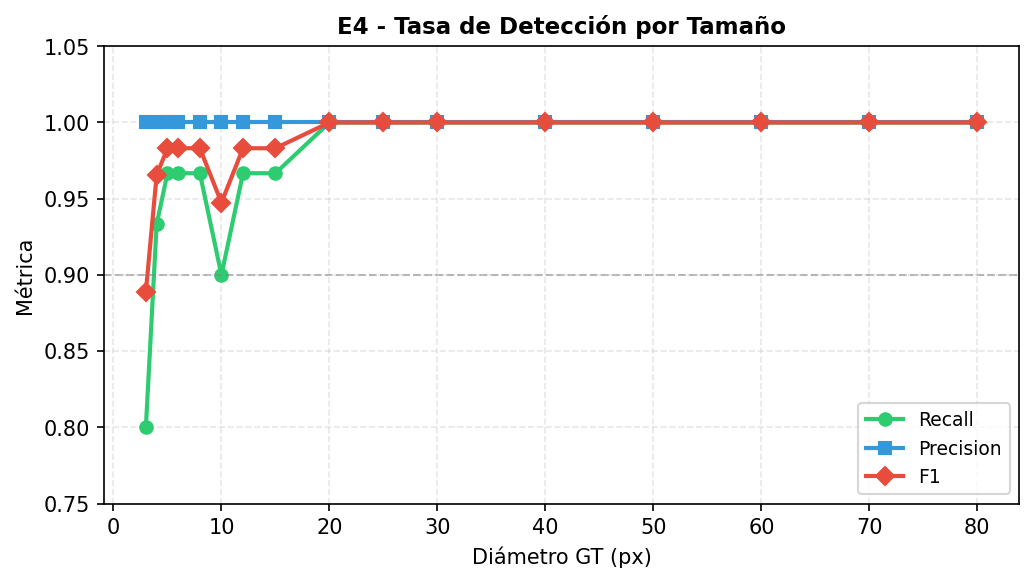
\includegraphics[width=\textwidth]{figures/tests/E4/E4_detection_rates.png}
    \end{subfigure}
    \begin{subfigure}[b]{0.85\textwidth}
        \centering
        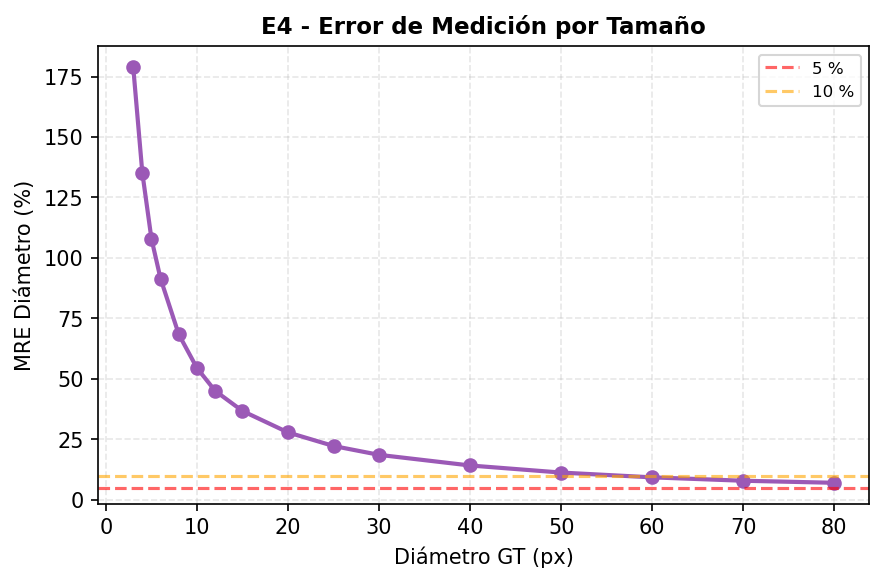
\includegraphics[width=\textwidth]{figures/tests/E4/E4_mre_diam.png}
    \end{subfigure}

    \caption{Métricas del experimento E4 (Rango de tamaños detectables).}
    \label{fig:E4_metrics}
\end{figure}

\subsection{E5 - Impacto de la densidad de gotas en el tracking}
 
\textbf{Configuración:} Se generaron vídeos de 60 frames con $N \in \{5, 10, 20, 35, 50\}$ gotas de 18~px de diámetro moviéndose simultáneamente a 3~px/frame en direcciones aleatorias (semilla fija para reproducibilidad), con ruido gaussiano de $\sigma = 8$. A mayor densidad, aumenta la probabilidad de oclusiones y de que el tracker asigne erróneamente la identidad de una gota a otra.

\begin{table}[H]
\centering
\small
\caption{Resultados del experimento E5 (impacto de la densidad de gotas en el tracking y la estimación cinemática). La Precision se omite por mantenerse constante en 1.0.}
\begin{tabular}{cccccc}
\hline
\textbf{Densidad ($N$)} & \textbf{Recall} & \textbf{F1} & \textbf{Fragmentación} & \textbf{MRE\textsubscript{vel} (\%)} & \textbf{RMSE\textsubscript{vel} (px/f)} \\
\hline
5  & 0.95 & 0.97 & 0.00 & 5.34  & 0.07 \\
10 & 0.91 & 0.95 & 0.10 & 5.47  & 0.09 \\
20 & 0.87 & 0.93 & 0.35 & 9.47  & 0.71 \\
35 & 0.81 & 0.89 & 0.31 & 16.90 & 1.12 \\
50 & 0.74 & 0.85 & 0.28 & 45.48 & 2.28 \\
\hline
\end{tabular}
\label{tab:e5_resultados}
\end{table}

En la Tabla \ref{tab:e5_resultados} y las figuras \ref{fig:E5_metrics} se cuantifica el deterioro del rendimiento del algoritmo a medida que aumenta la densidad de partículas. Como era previsible, el incremento en la concentración induce un mayor número de oclusiones espaciales, provocando una caída monótona en la tasa de recuperación (Recall), que desciende desde un excelente 0.95 con 5 gotas hasta un 0.74 en el escenario de máxima congestión (50 gotas). El efecto más perjudicial recae sobre el módulo de tracking y la estimación cinemática: a partir de las 20 gotas simultáneas, la tasa de fragmentación de trayectorias sufre un incremento abrupto (0.35). Esto indica que el algoritmo pierde la pista de las partículas durante los cruces y corrompe el cálculo temporal del desplazamiento, disparando el error relativo de la velocidad (MRE\textsubscript{vel}) por encima del $45\%$ en densidades extremas. No obstante, es crucial contextualizar estos resultados: en esta simulación sintética, las partículas se mueven en direcciones totalmente aleatorias, un diseño planteado ex profeso para someter al sistema a una prueba de estrés en el peor escenario posible. En un ensayo físico real de nebulización, el flujo posee una marcada direccionalidad, con la inmensa mayoría de las gotas viajando en el mismo sentido desde el inyector hacia el exterior. Esta coherencia vectorial reduce drásticamente la probabilidad geométrica de trayectorias cruzadas en comparación con el modelo sintético. Por tanto, aunque las estimaciones cinemáticas deben evaluarse con cautela en el núcleo más denso del aerosol, el rendimiento y la continuidad del tracker en condiciones reales de laboratorio serán previsiblemente superiores a los reportados en este límite teórico.

\begin{figure}[H]
    \centering
        
    \begin{subfigure}[b]{0.7\textwidth}
        \centering
        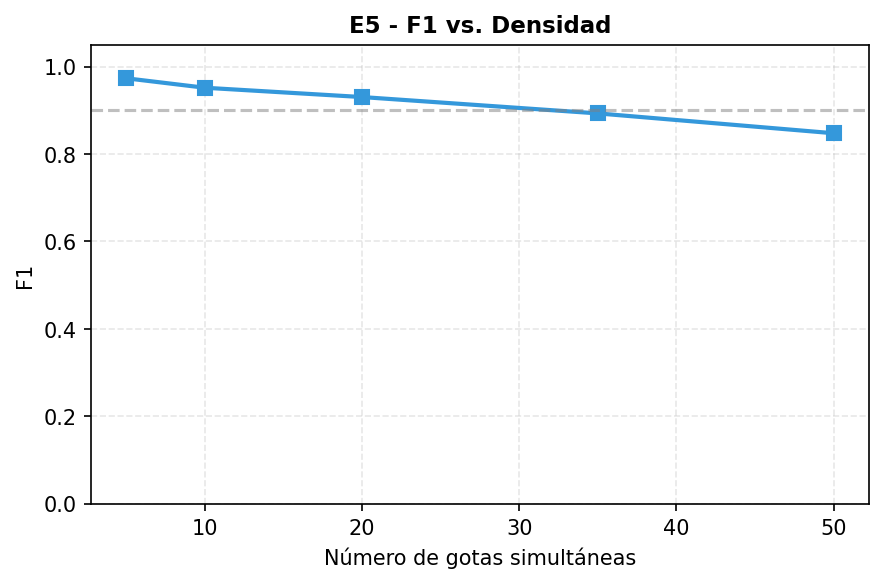
\includegraphics[width=\textwidth]{figures/tests/E5/E5_f1.png}
    \end{subfigure}
    \begin{subfigure}[b]{0.7\textwidth}
        \centering
        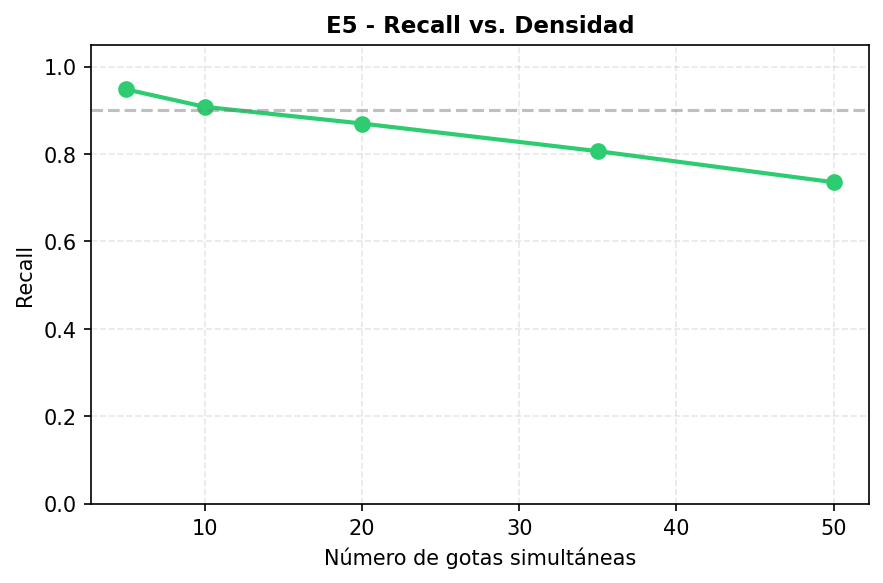
\includegraphics[width=\textwidth]{figures/tests/E5/E5_recall.png}
    \end{subfigure}
    \begin{subfigure}[b]{0.7\textwidth} 
        \centering
        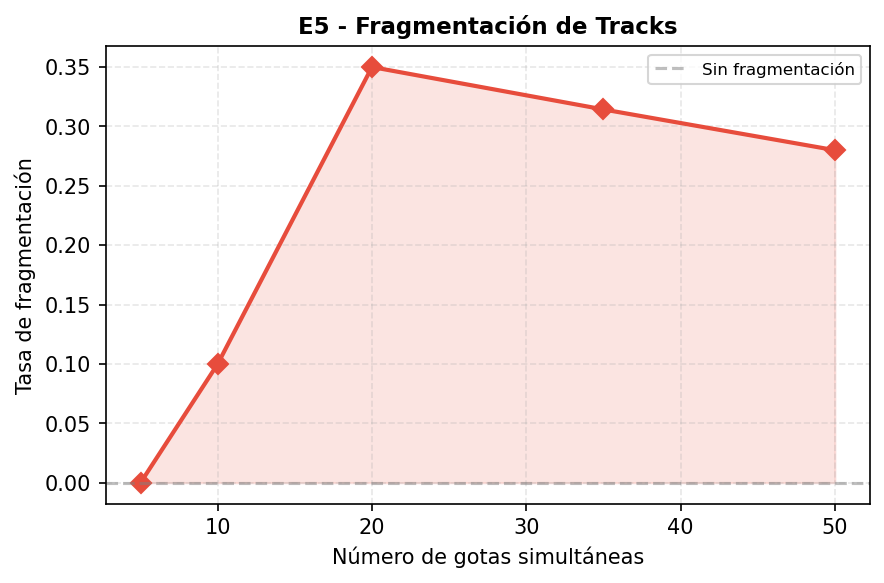
\includegraphics[width=\textwidth]{figures/tests/E5/E5_frag_rate.png}
    \end{subfigure}
    
    \caption{Métricas del experimento E5 (impacto de la densidad de gotas en el tracking y la estimación cinemática).}
    \label{fig:E5_metrics}
\end{figure}

\section{Evaluación cualitativa}

La evaluación cuantitativa sobre vídeos sintéticos valida la precisión del sistema bajo condiciones controladas, pero no garantiza su correcto funcionamiento con los vídeos reales de los experimentos de nebulización, que presentan características distintas: iluminación no uniforme, gotas desenfocadas en distintos planos, presencia del anillo circular del objetivo de la cámara y movimientos más complejos.

Para evaluar el desempeño del analizador en condiciones reales, se han procesado varios vídeos de experimentos de nebulización realizados en el laboratorio. En la figura \ref{fig:real_video} se muestra un frame de uno de estos vídeos, con las detecciones y tracks superpuestos.

\begin{figure}[H]
    \centering
    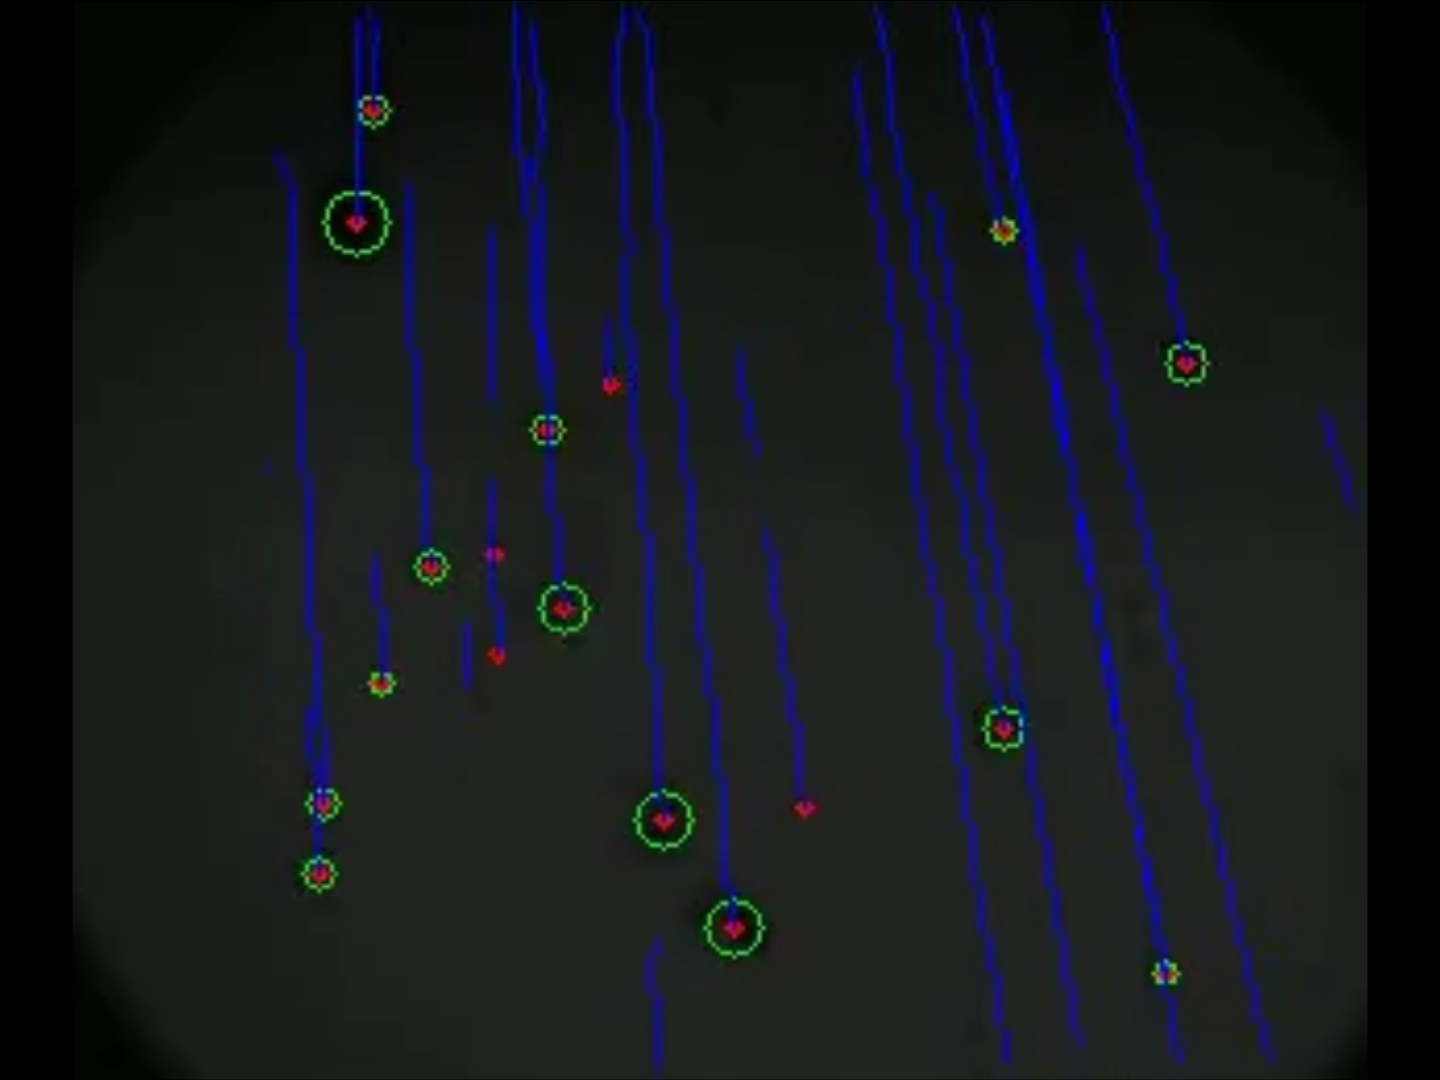
\includegraphics[width=0.8\textwidth]{figures/cuali.png}
    \caption{Frame de un vídeo real procesado por el analizador. Las detecciones se muestran como círculos verdes y los tracks como líneas de colores.}
    \label{fig:real_video}
\end{figure}

En el frame anterior se puede apreciar que pese a la baja calidad del vídeo se consiguen extraer la mayoría de las gotas junto con sus trayectorias. Además, las trayectorias marcadas, no poseen apenas discontinuidades, lo que indica que el analizador ha sido capaz de seguir el rastro de las gotas. Hay que decir, que hay gotas que no se detectan debido a la mala iluminación, el desenfoque y la oclusión, pero el sistema nos da una aproximación general de la dinámica del spray.
    \chapter{Conclusión y Trabajos Futuros}

    % Bibliografía
    \bibliographystyle{unsrtnat}
    \bibliography{bibliografia}
        

% Fin del documento
\end{document}
